\chapter{Experiment 2: Selection pressure}
\label{exp2}
In the original paper, Fernando et al. used a tournament search algorithm for path optimization. This algorithm was selected on the basis that it fills the role of simplest possible 'agent' for path-selection, one which can be considered a unit of evolution.  The tournament implementation fits this description as a 'unit' because of the tournament size used. Within one generation, the total change in the population is one genotype being replaced with another from the same population and subjected to mutation under some probability. Building on the previous set of experiments where the conclusion can take form as an argument in favour of a high exploration rate during path-search, we would expect a tournament of size two to yield modules with high transferability and a high number of reuse compared to a high tournament size. In these experiments, this will be tested by manipulating the selection pressure during the tournament search. Questions addressed in this section is: 
\begin{itemize}
    \item How would different evolutionary algorithms influence outcomes in training a PathNet structure on multiple tasks?
    \item What genetic programming strategies make the most sense in the scheme of training an SNN?
    \item How would a changing selection pressure affect learning? 
\end{itemize}
\newpage

\section{Description}
\subsection{Data-sets} \label{exp2:datasets}
To address these questions a trial of different searches have been applied to a PathNet structure for a selection of tasks. As with the first-path experiments, the search algorithms will be applied to image classification tasks. Building on what we learned with regards to task difficulty, two different data-sets have been selected, and the different tasks will be derived from this data. The tasks will be ordered by assumed difficulty to follow a gradual learning mentality. 

\begin{enumerate}
    \item MNIST subtasks
    \begin{enumerate}
        \item Digits 0, 1, 2, 3 and 4
        \item Digits 5, 6, 7, 8 and 9 
    \end{enumerate}
    \item Full MNIST classification
    \item Cropped SVHN subtasks
    \begin{enumerate}
        \item Digits 0, 1, 2, 3 and 4
        \item Digits 5, 6, 7, 8 and 9 
    \end{enumerate}
    \item Full cSVHN classification
\end{enumerate}

It was shown during the first-path experiments that task 1a and 1b is not of the same difficulty level, however, within this context we will consider the training amount needed to reach a satisfactory accuracy level is similar enough for these tasks to be grouped together. The natural progression from a full MNIST classification to a SVHN is thought to increase the incentive for module reuse, even if the SVHN task will have to learn to ignore distractions in the images (see \ref{Implementation:SVHN}) that the MNIST classifiers does not have to deal with. The difference in image-dimensions have been addressed in \ref{exp2:implementation}.

As mentioned in \ref{Implementation:SVHN} there are two formats to the SVHN set, one of variable image resolutions, and one that mimic the MNIST set in static square size called cropped SVHN (cSVHN). cSVHN is selected for these experiments in order to use a constant input size to the PathNet. Within the larger set of cSVHN images, a subset described as containing "somewhat less difficult samples" is used. To increase the number of tasks, the rest of the data in SVHN could be used and noise could be added to the images to increase the task difficulty artificially. 

For both the MNIST and cSVHN set, the amount of training data have been limited to 10000 training samples and 4000 validation samples. Of these samples, MNIST have an fairly even distribution on each class while SVHN have an imbalance in the class distribution. Since the samples used are randomly selected before each experimental run, the probability of select one sample from a given class can be derived from the total amount of samples in that class (see \ref{Implementation:SVHN} for the exact number of samples in each class).

Each experimental run will apply a searching scheme to find an optimal path in a gradually increasing knowledge base within a PathNet. This means, for instance, tasks 1a always will be learned in a module set of only initialized weights and no previous knowledge. It is assumed that with a different ordering in tasks, other  accuracy and training results would have been reached, but as this tells us more about the tasks selected than it does about the search algorithms used, and as each experimental run is significantly more time consuming than in the first-path experiments, this will not be attempted here. It is considered that this reversing of subtasks within a data-set partition could be used as an simple, if time consuming and crude data analysis tool.

\subsection{Algorithms}\label{exp2:algorithms}
The different versions of tournament search explored here have been divided into three groups: 
\begin{enumerate}
    \item Constant selection pressure
    \begin{enumerate}
        \item Tournament size 2
        \item Tournament size 25
        \item Tournament size 3 + recombination
    \end{enumerate}
    \item Scaling selection pressure
    \begin{enumerate}
        \item Low to high pressure: 2, 5, 10, 15, 20, 25
        \item High to low pressure: 25, 20, 15, 10, 5, 2
    \end{enumerate}
    \item Dynamic selection pressure
    \begin{enumerate}
        \item Gradual change from 2 to 25 over all generations
        \item Gradual change from 25 to 2 over all generations
    \end{enumerate}
\end{enumerate}
In total, the seven tournament algorithms are used 10 times each within a reinitialized PathNet structure to train on all tasks discussed in \ref{exp2:datasets}. Between algorithms, the only hyper-parameter change is the tournament size and replacement method within each tournament. All algorithms except 1c use a winner-replace-all scheme where the mutation of the strongest paths genome replaces each of the loosing contenders in the tournament. In algorithm 1c, three contenders are selected randomly from the population and evaluated. The two strongest genomes are labeled as parents and (starting with the winner) takes turns copying their layers to the offspring. The offspring is then subject to some mutation under the same probability as every other algorithm, and replaces the loosing genome in the tournament.
\begin{figure}[ht]
    \centering
    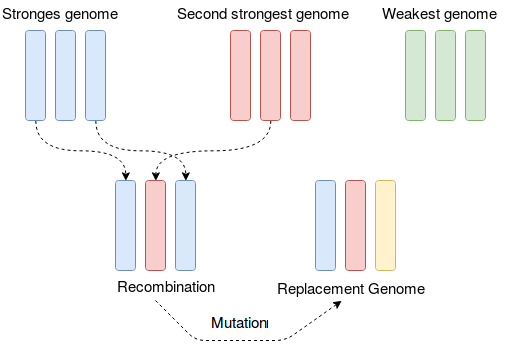
\includegraphics[width=0.8\textwidth]{Chapters/4.Experiments/exp2/figures/Recombination_algorithm.png}
    \caption{Visualization of the recombination in algorithm 1c. In a three layer PathNet, the first and last layer in the recombination would be layer one and three in the winning genome, while layer two would stem from the second strongest genome. After a mutation of the recombination, the new genome replaces the loosing contender. Each color represents one genome from the tournament and yellow represents a mutation.}
    \label{fig:search.recombination_algorithm}
\end{figure}

Algorithm group 2 consists of two algorithms where the tournament size is changed between each task. This means algorithm 2a uses tournament size 2 for task 1a, task 1b uses tournament size 5 and so on until the last task of full cSVHN classification which uses tournament size 25. In algorithm 2b, this order of tournament sizes is reversed. It is expected that in visualization of metrics where a population average is calculated for each generation, such as training accuracy, an algorithm with high selection pressure will have abrupt value changes from one generation to the next. Low selection pressure would then give a more gradual change in such values. A change between these two curve types should be prominent for algorithms 2a and 2b.

Algorithms 3a and 3b have its selection pressure changed during each tournament search. This means each algorithm behave the same for each task, which algorithms 2a and 2b did not. The change in selection pressure is gradual which means between tournament sizes 2 and 25, each tournament size is used about 4 times for a search termination limit of 100 generations. It is obvious that an even distribution of tournament sizes on each generation is not possible when using a threshold accuracy as search termination, which is one reason searches in these experiments are limited by number of generations instead. 

\subsection{Metrics}\label{exp2:metrics}
Due to the experiment complexity and number of tunable hyperparameters there are a large number of search effects and attributes that could be investigated, so limitations have been introduced on which metrics are being addressed. 

As with the first-path experiments, module reuse between tasks will be an important metric. This number is highly effected by stochastic processes such as initialization of populations, mutation probability, layer sizes, path sizes and so on, but it is also the most intuitive and clear way to measure the transferability of module knowledge. An assumption used behind this metric is that modules are able to contain some form of "memetic"\footnote{Memetic is used here to describe a quantification of knowledge in the same way "meme" is used by Richard Dawkins\cite{selfishGene} to describe a unit of cultural knowledge} unit knowledge. In this multi-task scenario, reuse can occur across multiple tasks, but focus will here be put on the total number of modules reused instead of separating the reuse across tasks. This is because any effect algorithm choice has on module reuse will be compounded and easier to spot in the total amount of reuse rather than in reuse between tasks.
%ABRIDGED: This is because if the effect on reuse between each search algorithm is small, the stochastic noise in reuse on between two tasks is not as descriptive of how an algorithm affects learning as with the total number. 

This reuse can indirectly be seen by viewing the total number of modules used for all tasks. This total capacity use is both a result of the reuse of modules and the path size. Which means capacity could be used as a measure of how "effective" the learning under a search algorithm is. By using few modules in each task and reusing a high number of modules from previous tasks, little new parameter optimization have to be done. This effective parameter use would possibly reduce the overall validation accuracy so in order to visualize the effectiveness of training, total number of training units applied to each module in each path would be a useful metric. 

To confirm the ordering of algorithms on the exploration/exploitation scale, a population diversity metric will be calculated\footnote{See \ref{background:diversity} for more details about how this is computed} for each algorithm. The reduction in this diversity for each generation gives an indication of the convergence-rate of each algorithm. Those of high exploitation will quickly hone in on one genotype and optimize the weights along that path, while algorithms that focus on exploration will explore many more permutations of modules. 

During a search for an optimal path as solution to a given task, the total training effort spent on the task is spread across the modules available for training. This means when the search is terminated and the optimal path have been locked to future back propagation, most of the updated parameters are lost due to the re-initialization of open modules. While total computational efficiency is not something addressed in this thesis, the ratio of used training effort to the total training spent on a task is an interesting metric. This ratio is highly dependent on how quickly a population converges to one optimal path. In scenarios where this occur fairly early on in the lifetime of the search, every subsequent generation performs training where almost all is along the optimal path. We would therefore expect algorithms with a high selection pressure to be placed high in a ranking of useful training. See \ref{exp2:implementation} for description of a training unit. 

\section{Hypothesis}
\label{exp2:hypothesis}
The expectations for these experiments were heavily influenced by the results in the first-path experiments. When the training algorithms are viewed in a simplified context of only "exploration vs exploitation", we can place them on a scale between these extremes and discuss expected outcomes from each end of the spectrum. In this context, the Pick+Search learning scheme used in the first-path experiments would fall on the exploitation side.

During a search, a given algorithm reduces the population diversity from a initialized state of high diversity until some optimal path is found. This convergence rate, and therefore also population diversity, is determined by which end of the exploration/exploitation spectrum we select our algorithm from. Since we limit ourselves by only changing the tournament size, we would expect a lower tournament size to lead to a low convergence rate and high diversity. This is a natural assumption to make considering the maximum change that occur in the population from one generation to the next. A tournament search with size two has such a low selection pressure that from one generation to the next, only one instance of genotypic change is applied the the population\footnote{This is when the weakest genotype is replaced by the winner of the tournament}. The number of generations until the population have converged to one optimal path would therefore be higher under such a search than a search where the selection pressure is considerable higher. 

A high selection pressure means strong phenotypes are favoured during the search. The algorithm would after one generation have a significant portion of its population genetically identical, ignoring possible genotypic traits caused by mutations. In the search context of finding an optimal path in a PathNet structure, evaluating a lot of similar paths to rank their fitness would lead to training the same modules multiple times. The next generation would then have a disproportionate fitness scores for some paths which would cause them to have a higher likelihood of winning the next generations tournament, and therefore quickly take control of a population by out performing all other paths. In such a scenario, the population have converged before other paths would have had time to adapt to pretrained modules interfaces, and the advantage PathNet brings with module transferability have been reduced, if not lost.  

For the locked tournament sizes the expectations are that high selection pressure causes high convergence and low module reuse between tasks. The low reuse would again cause more of the total number of modules in the PathNet to be locked after all tasks are learned. What the pressure would mean for validation accuracy is highly dependent on what tasks are learned, and from which domains they are selected. 
The opposite is true for the searches with a small tournament size. The low convergence leads each module to be trained in multiple permutation of PathNet subsets, and therefore also more transferable than modules trained during high selection pressure. If the searches are limited by the number of generations, and not by a threshold training accuracy, it would not be a surprise if the high tournament sizes yields paths with a higher validation accuracy for each task than those searches with low selection pressure. This is because each generation contain more effective training when there are more genotypes in the tournament. Not to be forgotten is the fact that all paths in all generations have the same final task-specific layer.  Since this is shared across all paths, the high tournament sizes leads to orders of magnitude more training in the final layer for high selection pressures. For each generation, the final layer is trained once for each genotype being evaluated. Meaning after a hundred generations, it have been trained 1 order of magnitude more for a search with tournament size of 25 versus a tournament size of 2. 

In addition to the static tournament sizes with a winner-replace-all crossover scheme, a search with recombination is tried together with tournament size three.  This should give a selection pressure even lower than that of tournament size two. From one generation to the next, there is still only one genotypic change in the population, but where the normal tournament search replace the loosing genotype with the winner, a recombination of the two strongest phenotypes replaces the weakest genome\footnote{With some additional mutation}.  Another way to view the step from algorithm 1a to algorithm 1c is one with focus on the genome in the offspring that takes the weaker paths place in the population. Given the recombination scheme, it can be seen as a copy of the tournament winner, but with a strong mutation probability that is scaled down during the search. This down scaling comes from the convergence of the population. When the diversity is reduced, more and more paths will have a similar subset of modules. When selecting two paths with the same modules, the recombination will yield a path identical to both parents. So as a population grows closer to converging to an optimal path, it will consist of similar genomes and each recombination will give offspring closer to the population median than it would in a diverse population. 
In summary, a high tournament size is expected to shift the search algorithm in the direction of high exploitation which in turn should give a high performance on the different tasks. Low tournament sizes gives a high exploration of the different paths possible, which yields modules trained in multiple permutations of PathNet subsets. It is expected that this will lead to more module reuse, and generally have a lower capacity usage than algorithms of high selection pressure. 

It is hard to tell how the validated classification accuracy on the final task will be affected by the different algorithms. As with the previous experiments, the tasks selected might prove to be to simple which would hide much of the potential in transfer learning since a path of average since should be able to learn each task \textit{tabula rasa}.

\section{Implementation}
\label{exp2:implementation}

\textbf{Edit note: Compare implementation to that of DeepMind for similar task (cifar vs SVHN)}

\subsection{PathNet}
The PathNet structure used for these experiments have three layers of 20 modules where each path may contain one, two or three modules in each layer. The 20 modules were selected to make sure there would be a non-zero probability of selecting only empty modules for all tasks, even if all optimal tasks contained the maximum number of modules without any module overlap between tasks.

As with the refined first-path experiments, only convolutional modules with ReLU activation were used, but with two channels each instead of the one in first-path. To verify, a random path with these hyper-parameters were created and applied to the task of full cSVHN classification and was able to reach a satisfactory performance within a reasonable training time. The Adam optimizer were used during back propagation with a learning rate of 0.0001. 

Each convolutional module also includes a batch-normalization operation and the last modules ends in a max-pooling before the output is flattened and passed through the final unique classification layer. 

\subsection{Image-sets}
As there is a resolution difference between the cSVHN set and MNIST, an additional preprocessing step were applied to the MNIST set. A 2 pixel border of zeros were added to change the dimensions from 28x28 to 32x32. cSVHN images has three-channels of RGB values so the single channel of padded MNIST images were repeated in every color-channel to reach the final dimensions of 32x32x3.  

\begin{figure}[ht]
    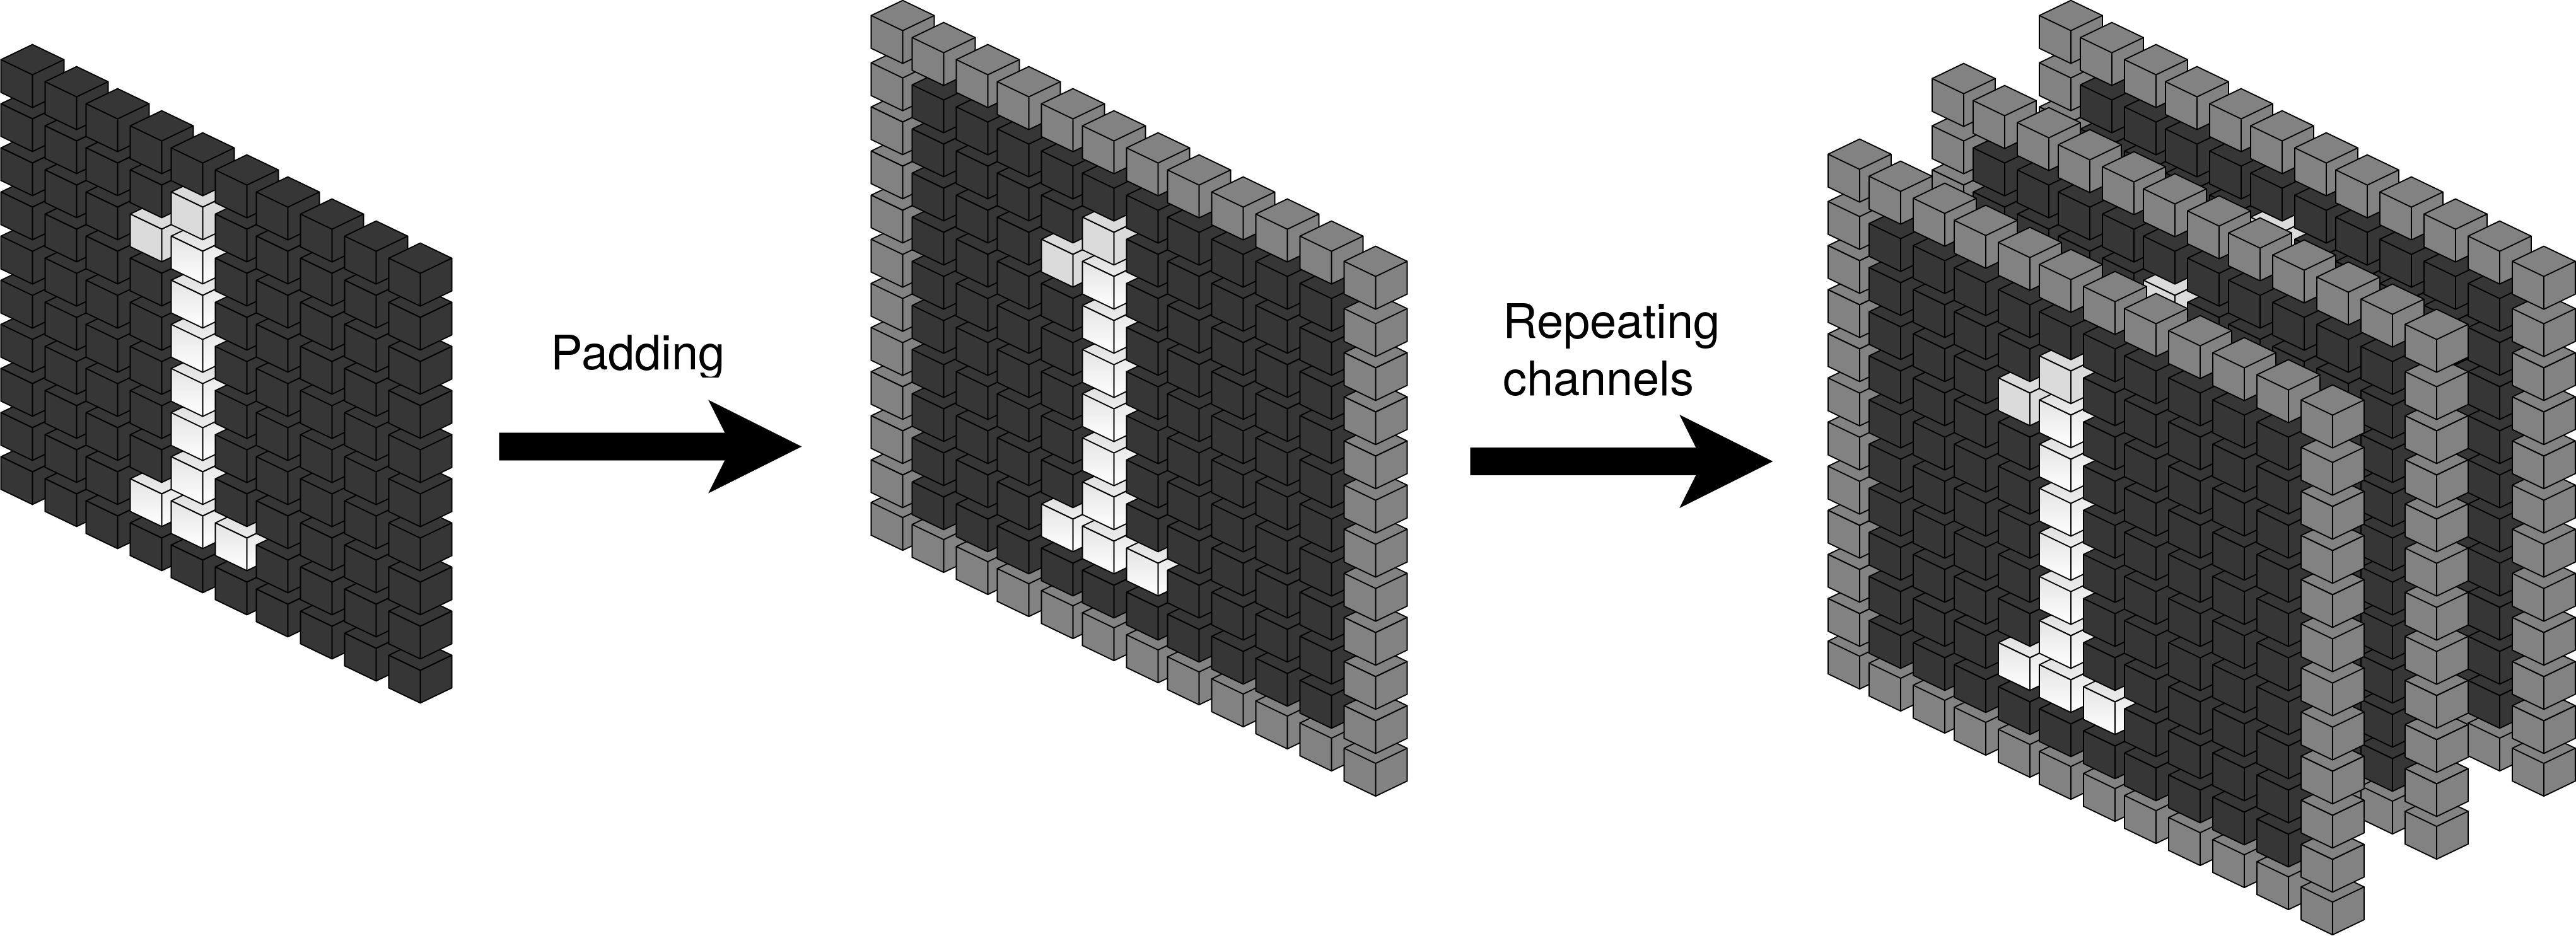
\includegraphics[width=\textwidth]{Chapters/4.Experiments/exp2/figures/MNISTpadding+repeating.png}
    \caption{How MNIST is adapted to have same dimensions as cSVHN. Illustration use dimensions 12x12x3 while cSVHN and adapted MNIST use 32x32x3}
    \label{fig:MNISTpadding}
\end{figure}

\newpage

\subsection{Tournament Search}\label{exp2:implementation.search}
The tournament search uses a population size of 64, and as discussed, a winner-replaces-all replacement scheme between generations. Instead of using a accuracy threshold as in the previous experiments, the search terminates after 100 generations. A important feature of PathNet is the way learning is done. Since network back propagation occur during path fitness evaluation, the locked number of generations limit the amount of training that is allowed. In the original paper, fitness is set as the negative training error which is reached for each path after it have been trained for one training unit of 50 mini batches of size 16. This is an reasonable way of evaluating the fitness of a path when using a small tournament size, but as the tournament size have been increased tenfold for the algorithms with high selection pressure, fitness is calculated differently in these experiment. 

The problem of directly using the training error as fitness is that the error changes whenever weights along a path is updated. An extreme example can be used to present the underlying problem with this.

\begin{figure}[ht]
    \centering
    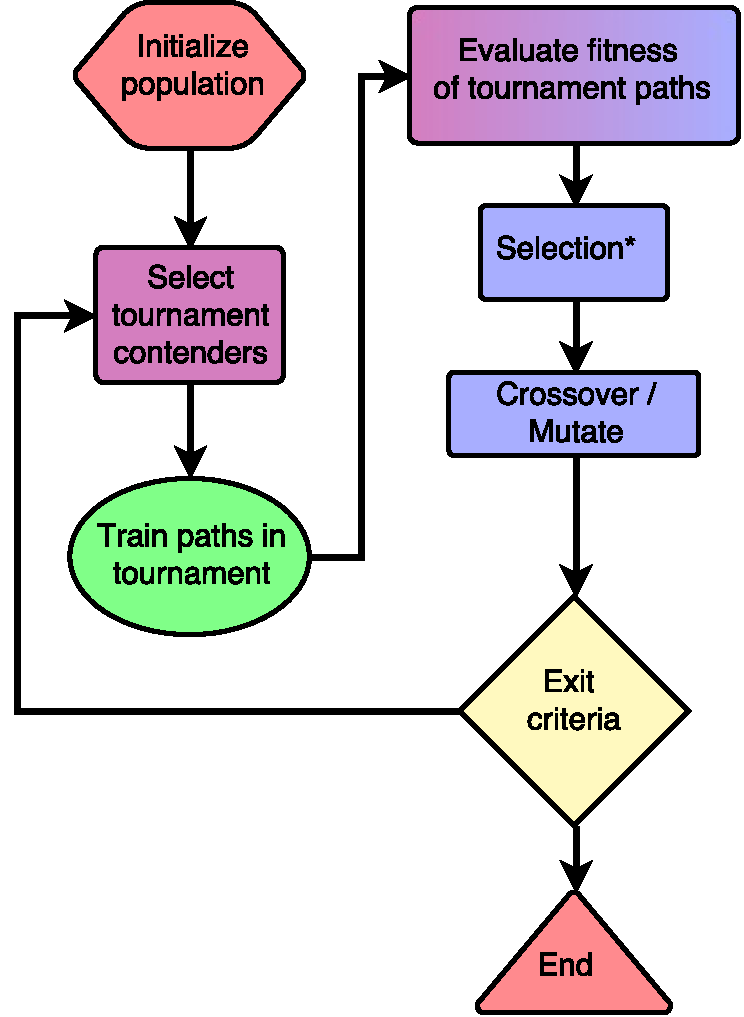
\includegraphics[width=0.5\textwidth]{Chapters/4.Experiments/exp2/figures/TS_implementation.pdf}
    \caption{Flowchart of the tournament search implemented here. Compared to the flowchart of standard Tournament Search implementation in figure \ref{fig:algorithmflowcharts}, the difference is the extra step of training (green) before the fitness is evaluated. *The selection function always selects the tournament winner, except during algorithm 1c where the top two paths is selected.}
    \label{fig:ts_flowchart}
\end{figure}

Take a tournament selection of 25 genomes containing 24 identical paths and one different path with some module overlap to the others and which is evaluated first. One scenario could be that the first unique path is evaluated to a high fitness, when the next path evaluated, the weights in the modules which overlap between the two are updated. The evaluated fitness of the first path is now outdated, and for every subsequent path, this fitness might get worse and worse if the parameters in the overlapping modules move to an area of high error in the context of the first paths other modules. After all fitness evaluations, the first path now stands with a high fitness, which might be larger than that of all other paths in the tournament. Then all other paths in the tournament is replaced with the winning path even if its actual fitness might have become significantly reduced during the evaluation step. Due to this, the fitness of paths in a tournament is calculated in a separate step for these experiments as seen in figure \ref{fig:ts_flowchart}. After a subset of the population is selected for a tournament, all paths in that tournament are trained for one training unit. When training is completed, each path is evaluated by using a new subset of the training data for validation. This way, the order in which paths are validated does not affect the fitness score, which is the classification accuracy reached during the validation step. The order of paths still affect the the training but the fitness used for selecting a tournament winner is the "true"\footnote{Fitness is still calculated on the basis of the training data-set, which means it might become overly optimistic over time. Overfitting during training is discussed in the context of another experiment} fitness score.

The same reason influence the final step of the tournament search. When the limit of a hundred generations is reached, all paths in the population is evaluated again. Since the true fitness of a path might change from one generation to the next, only the paths participating in the final tournament has its true fitness score as part of the selection of the optimal path. As with the evaluation step, the final fitness of a path is the reached classification accuracy of one training unit (50 mini-batches of 16 samples). Using an actual validation set for this step might yield better, or at least more accurate, fitnesses to use as a basis for path-selection, but that would significantly increase the run-time of an already time intensive experiment. 

\section{Results}
\label{exp2:results}
Due to the experimentation being time-consuming, each algorithm were run 10 times and logs were saved after each experimental run of each algorithm. The following plots have been separated in three groups based on subject: paths, search and training. 

\subsection{Paths}
To test the effect algorithm choice has on path size, MWW tests (see appendix \ref{background:mannwhitney}) were run to test the null hypothesis that a pair of algorithms have the same path size distributionn. The resulting p-values are presented in the tables in section \ref{appendix:ptable.pathsize}. Using the Bonferroni corrected \(\alpha\) level of 
\begin{equation*}
    \alpha=\frac{\alpha_{desired}}{\text{number of MWW tests}}=\frac{0.05}{126}=3.968\time 10^{-4}
\end{equation*}
none of the null-hypotheses can be rejected, meaning the algorithm choice have no affect on path size. 

Also tested are the null-hypotheses that a algorithm A have the same distributions of total capacity used as a algorithm B for both A, B \(\in [1a, 1b, 1c, 2a, 2b, 3a, 3b]\) and A \(\neq\) B. Each algorithms capacity-use is also compared to the Monte-Carlo estimate, making 28 Mann-Whitney tests necessary. A significance level of \(\frac{0.05}{28}=1.7857\time 10^{-3}\) is therefore used. For this \(\alpha\) (or indeed a standard \(\alpha=0.05\). See table \ref{tab:exp2.capacityptable}) none of the algorithms were different from each other, but every algorithm was proved to be significantly different from the Monte-Carlo estimate of random capacity use. 

As a metric by itself, the capacity is influenced both by path-size and module reuse. All paths being equal, a high level of reuse for one algorithm would yield a significant difference in used capacity as the total number of used modules is reduced. As this is not observed we would expect the mean reuse for each algorithm to not contain significant differences.

\begin{sidewaysfigure}[p!]
    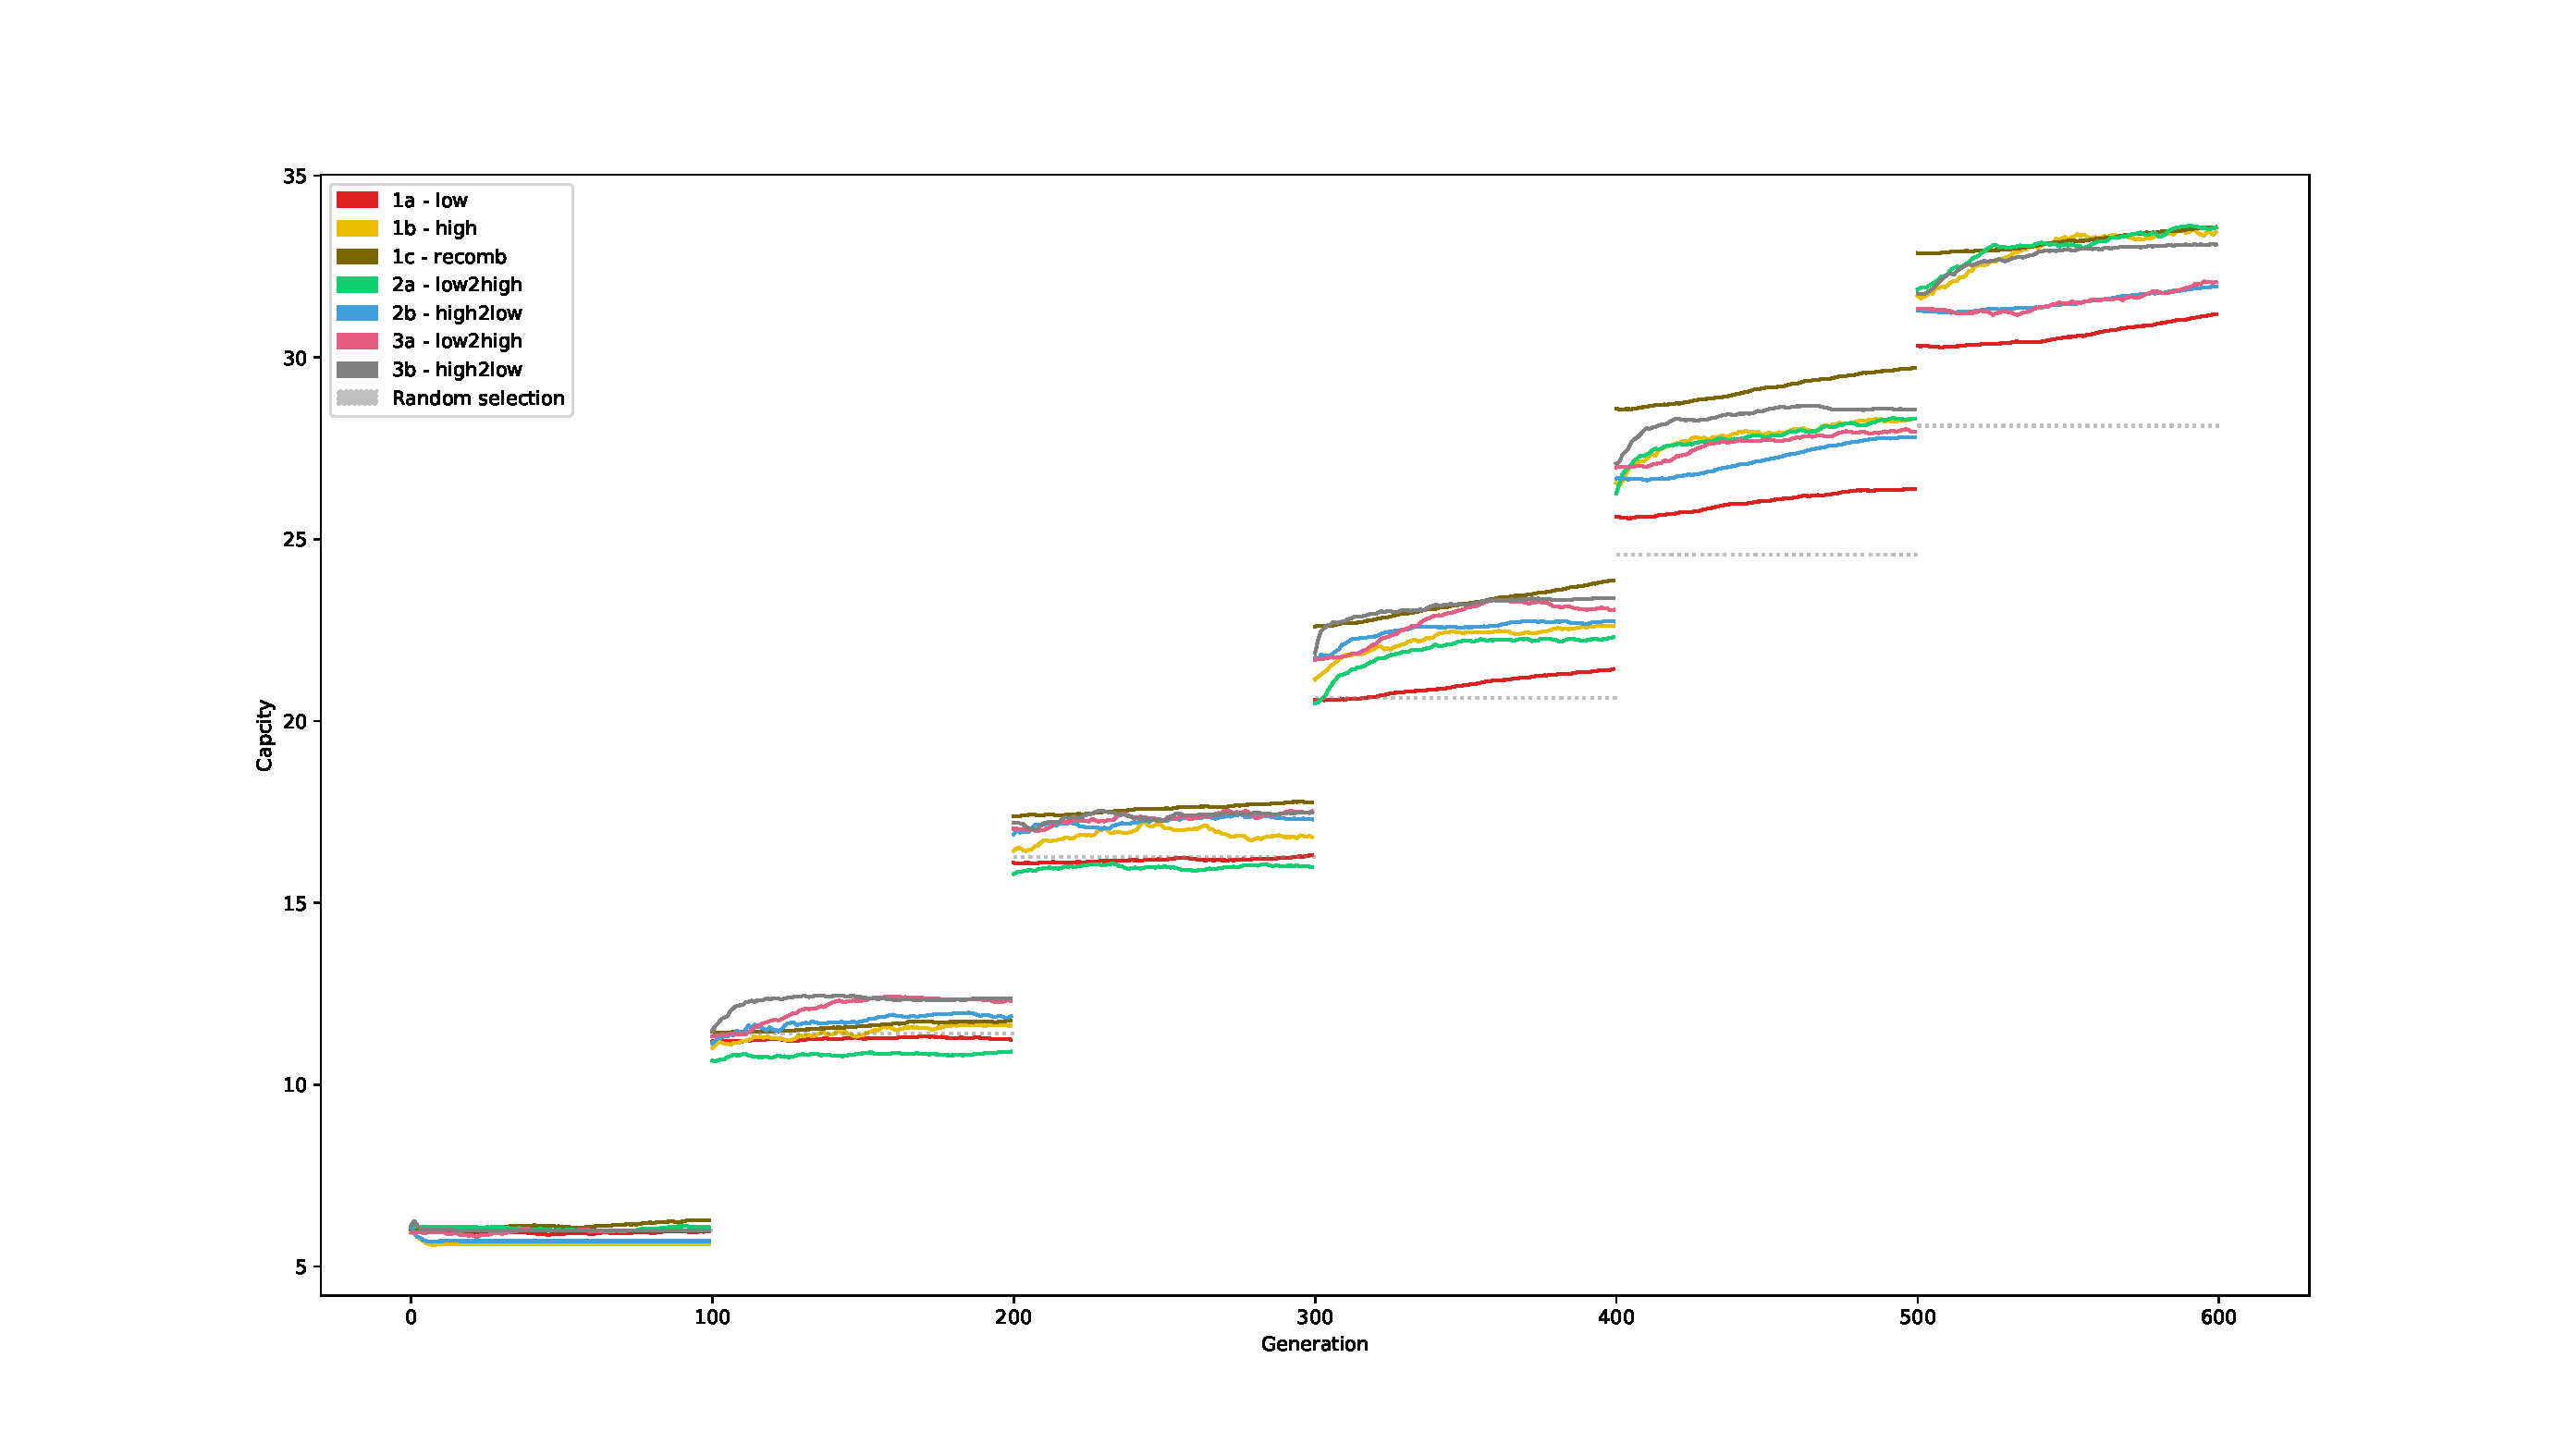
\includegraphics[width=1.2\textwidth,center]{Chapters/4.Experiments/exp2/figures/large/Capacity_pr_generation.pdf}
    \caption{The average number of used modules during the multi-task learning sequence. Each jump is caused by the saving of an optimal path and then starting a new search for a new task. }
    \label{fig:search.capacity}
\end{sidewaysfigure}

\begin{sidewaysfigure}[p!]
    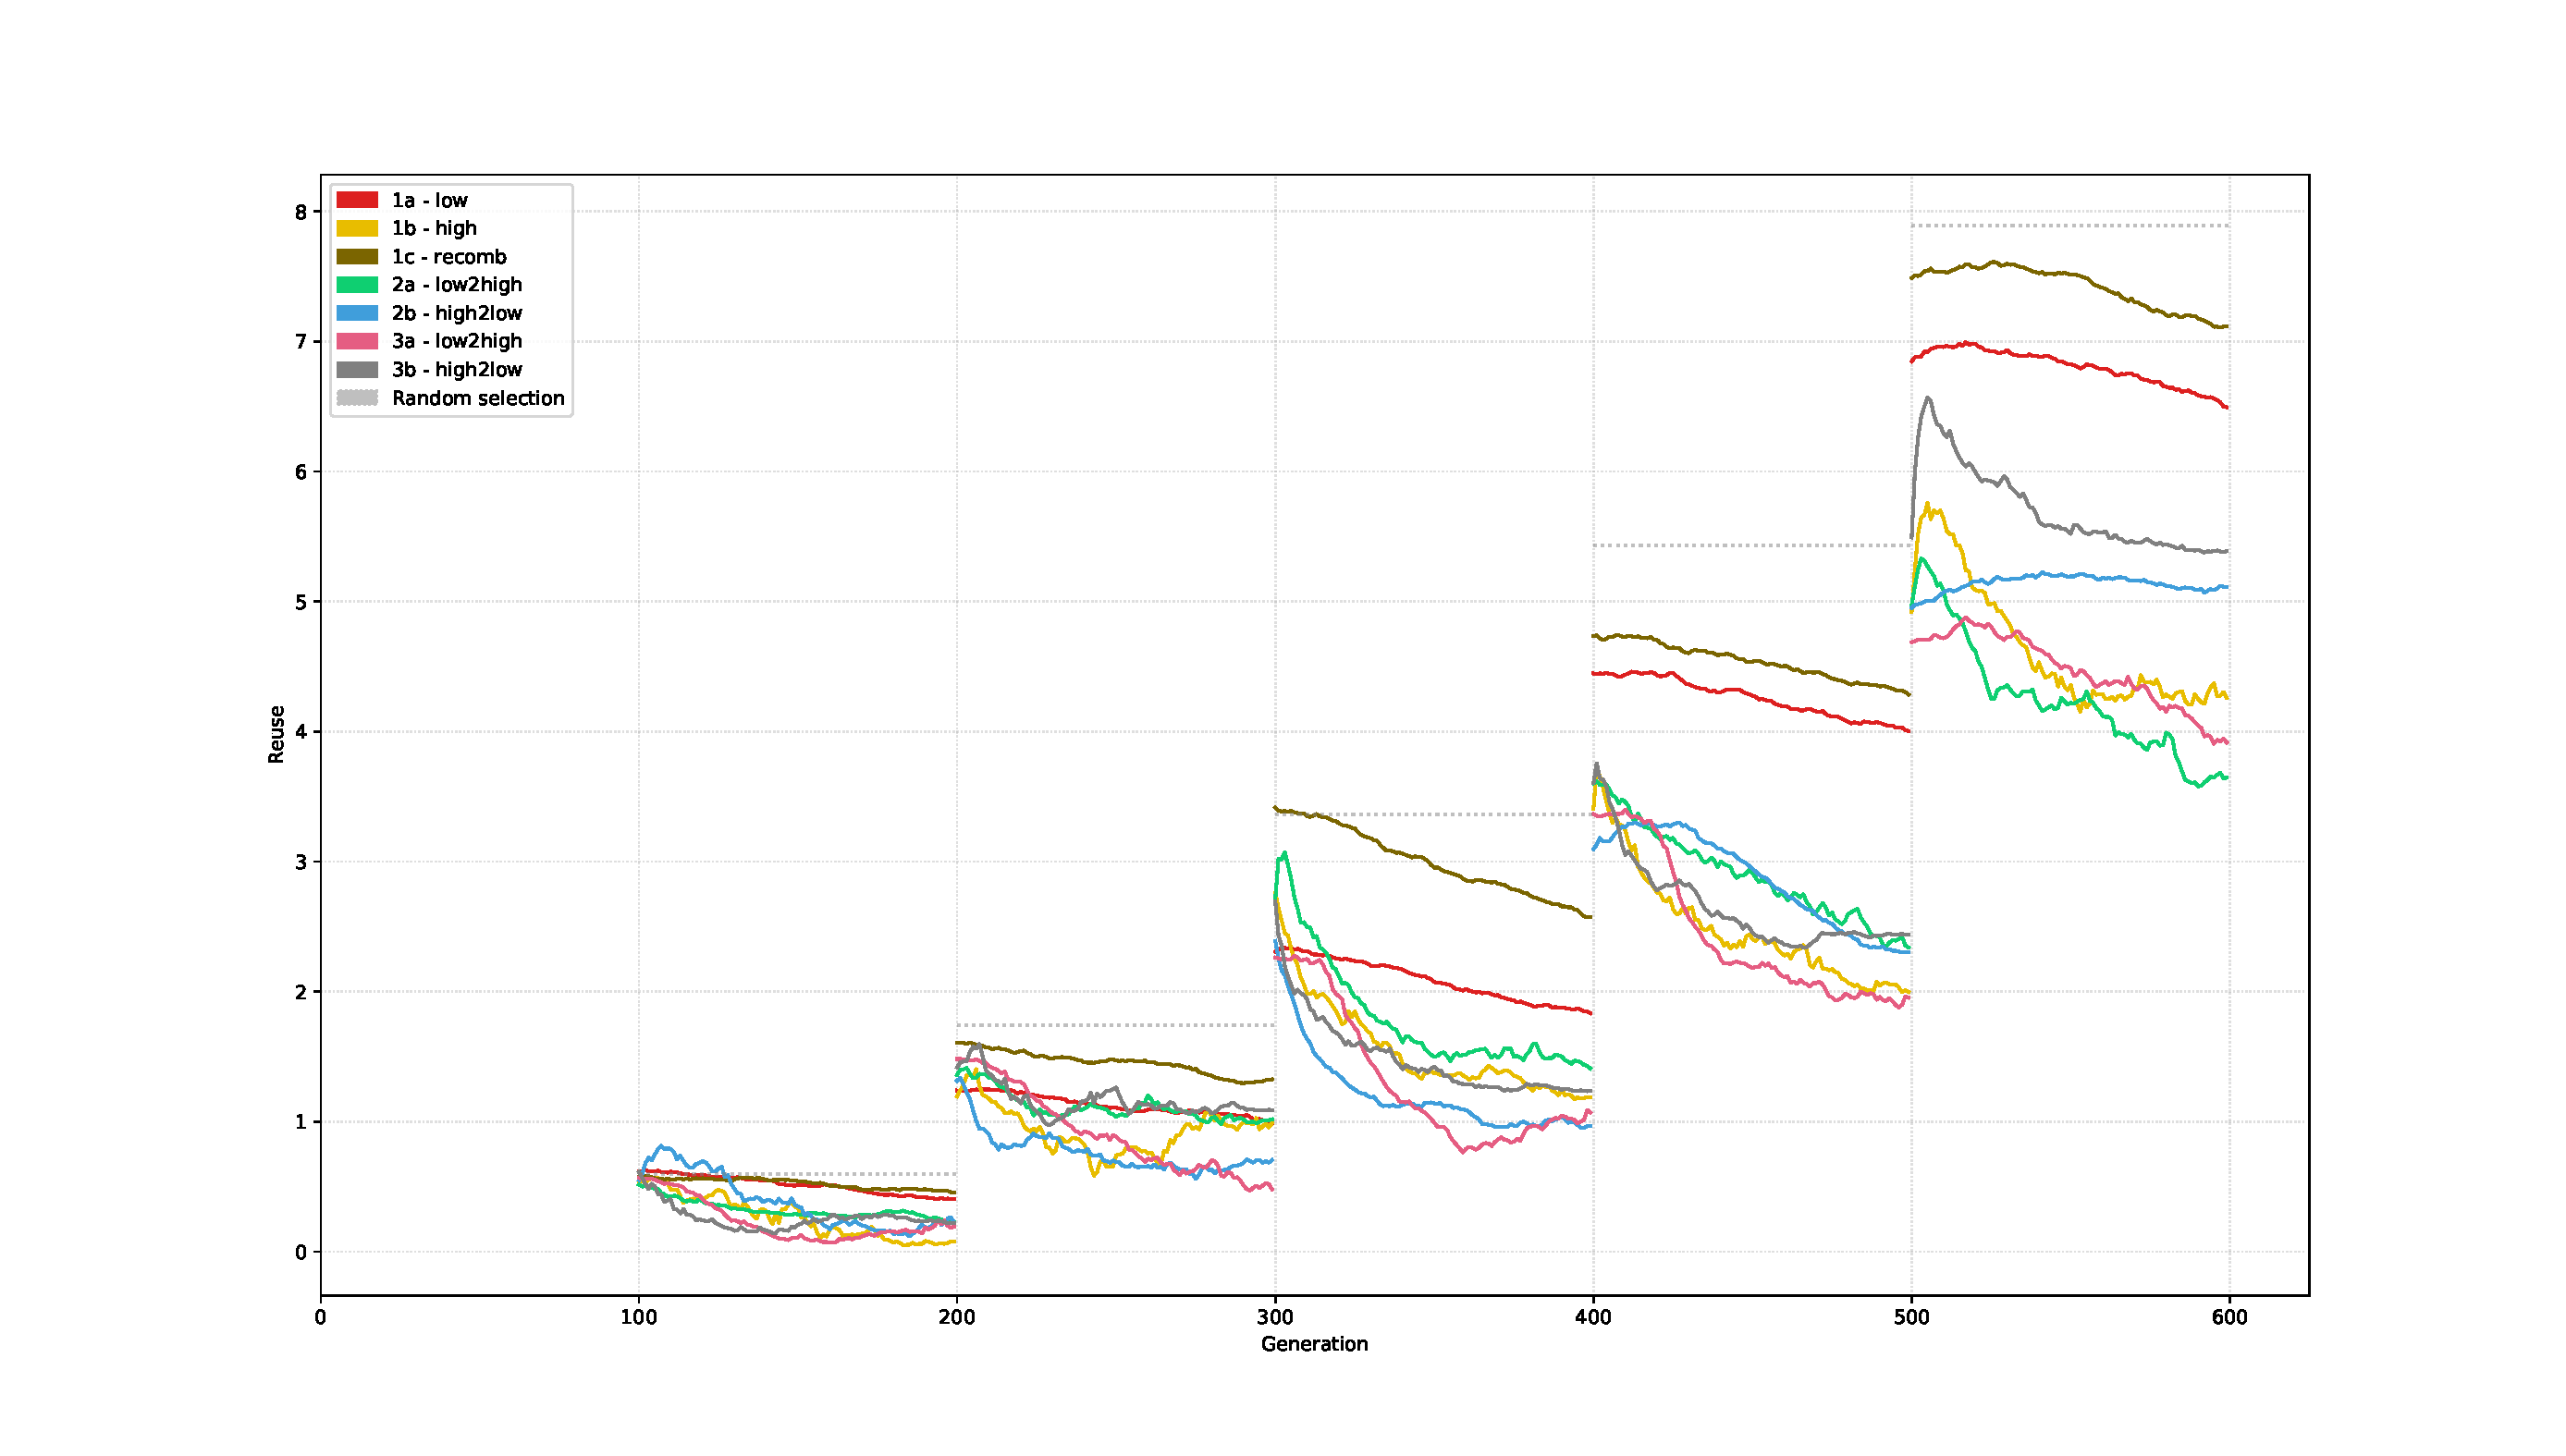
\includegraphics[width=1.2\textwidth,center]{Chapters/4.Experiments/exp2/figures/large/Module_reuse_pr_generation.pdf}
    \caption{The average module reuse during the multi-task learning sequence. Each jump is caused by the saving of an optimal path, and the next task having more locked modules to reuse. The first 100 generations does not have any previously learned knowledge to reuse.}
    \label{fig:search.reuse}
\end{sidewaysfigure}

Figure \ref{fig:search.capacity} underlines the MWW results as there is only a small visual difference in average capacity between the algorithms.  Figure \ref{fig:search.reuse} on the other hand contain escalating fluctuations in the mean reuse across each algorithm. While all are below the Monte-Carlo estimated reuse, the algorithms seem to affect the change in reuse within each search differently. Another round of MWW tests however disproves this (see table \ref{tab:exp2.reuseptable}) as no null-hypotheses could be rejected under the Bonferroni corrected \(\alpha\)-level.

\subsection{Population Diversity}
\ref{fig:search.hamming_diversity} visualizes the average population diversity for each algorithm for each task calculated with the pair-wise Hamming distance metric. As this metric is dependent on the size of population as well as the number of genes in a genotype, the value at one point in the generation is not depictive of anything, but instead, the overall trend of the measure indicates at what rate the algorithm converges. 

\begin{sidewaysfigure}[p!]
    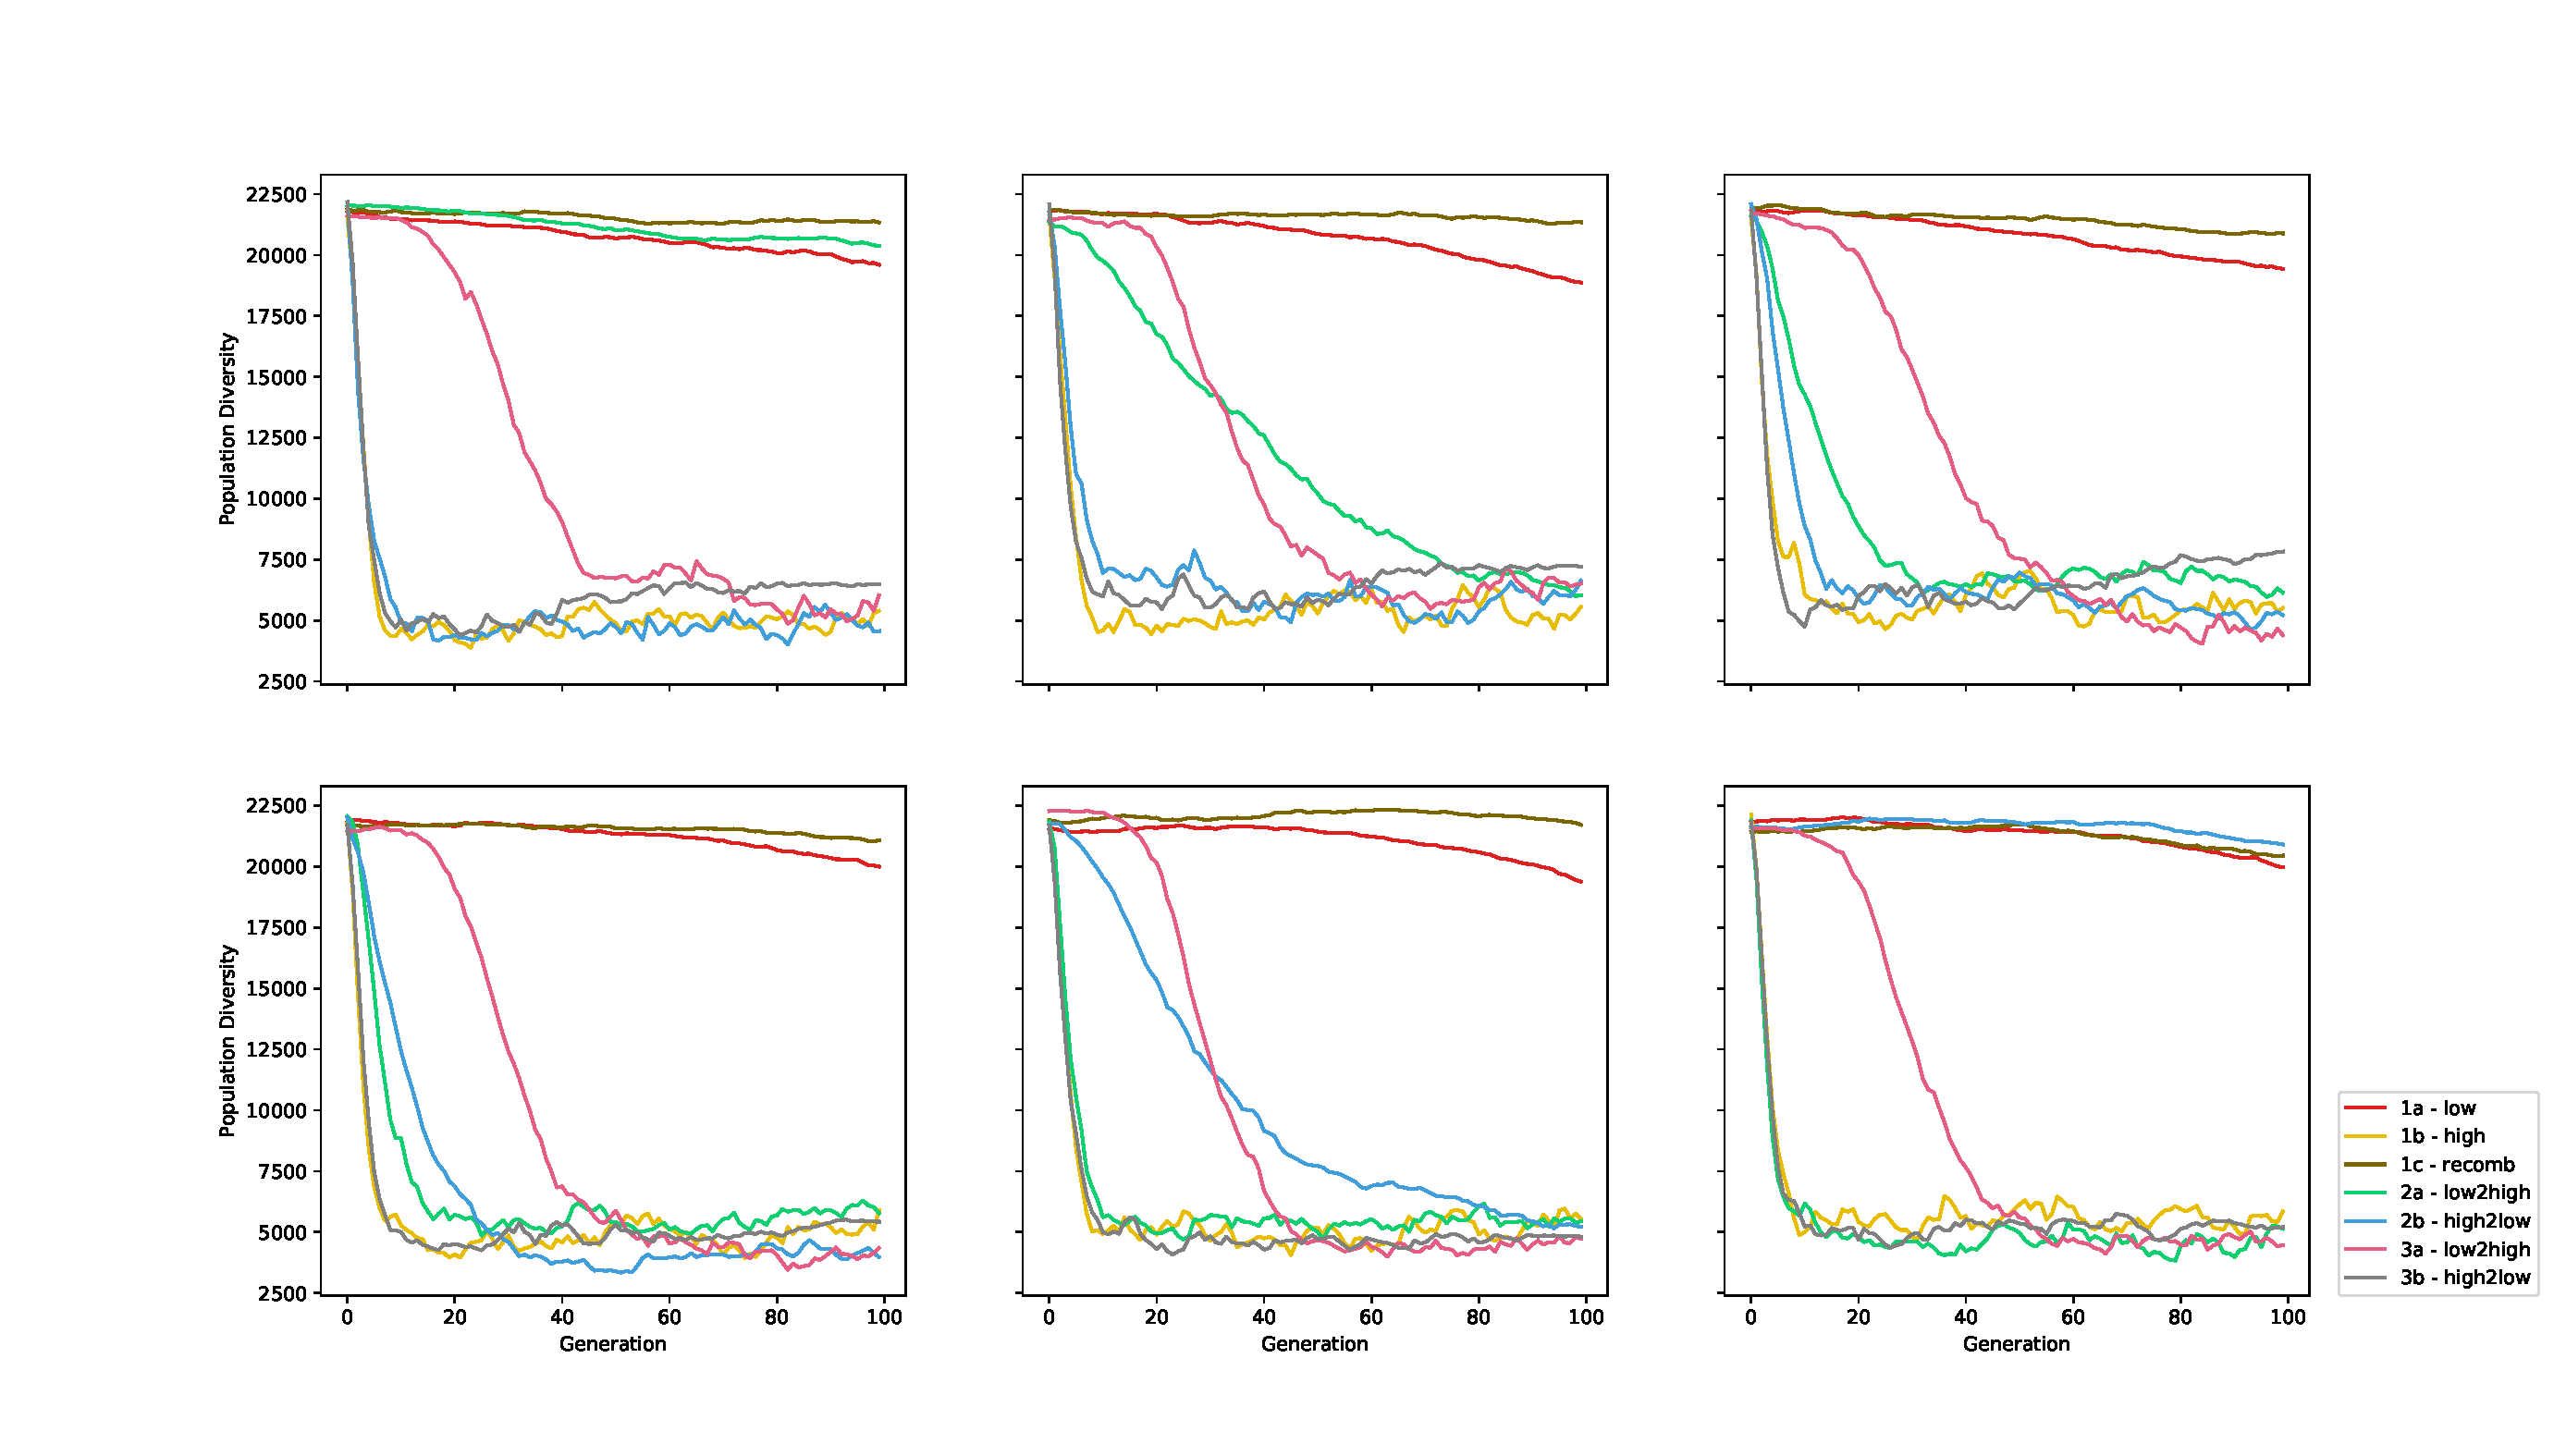
\includegraphics[width=1.2\textwidth,center]{Chapters/4.Experiments/exp2/figures/large/Average_population_diversity_reduced_hamming.pdf}
    \caption{The average pairwise Hamming distance within each generation is used as a measure for population diversity. Each subplot (in order left to right) is each task in trained order.}
    \label{fig:search.hamming_diversity}
\end{sidewaysfigure}

When a generation is over and mutations of the tournament winner replace all losers, the population makes a large shift in diversity unless most of the tournament participants have a similar genome, at which point population have most likely converged. This is why all diversity plots (\ref{fig:search.hamming_diversity} and \ref{fig:search.frequency_diversity_unique}) contain rapid changes for sections of high tournament size, while algorithms 1a and 1c (also algorithm 2a for the first tasks, 2b for the later tasks) have more gradual changes. 

\begin{sidewaysfigure}[p!]
    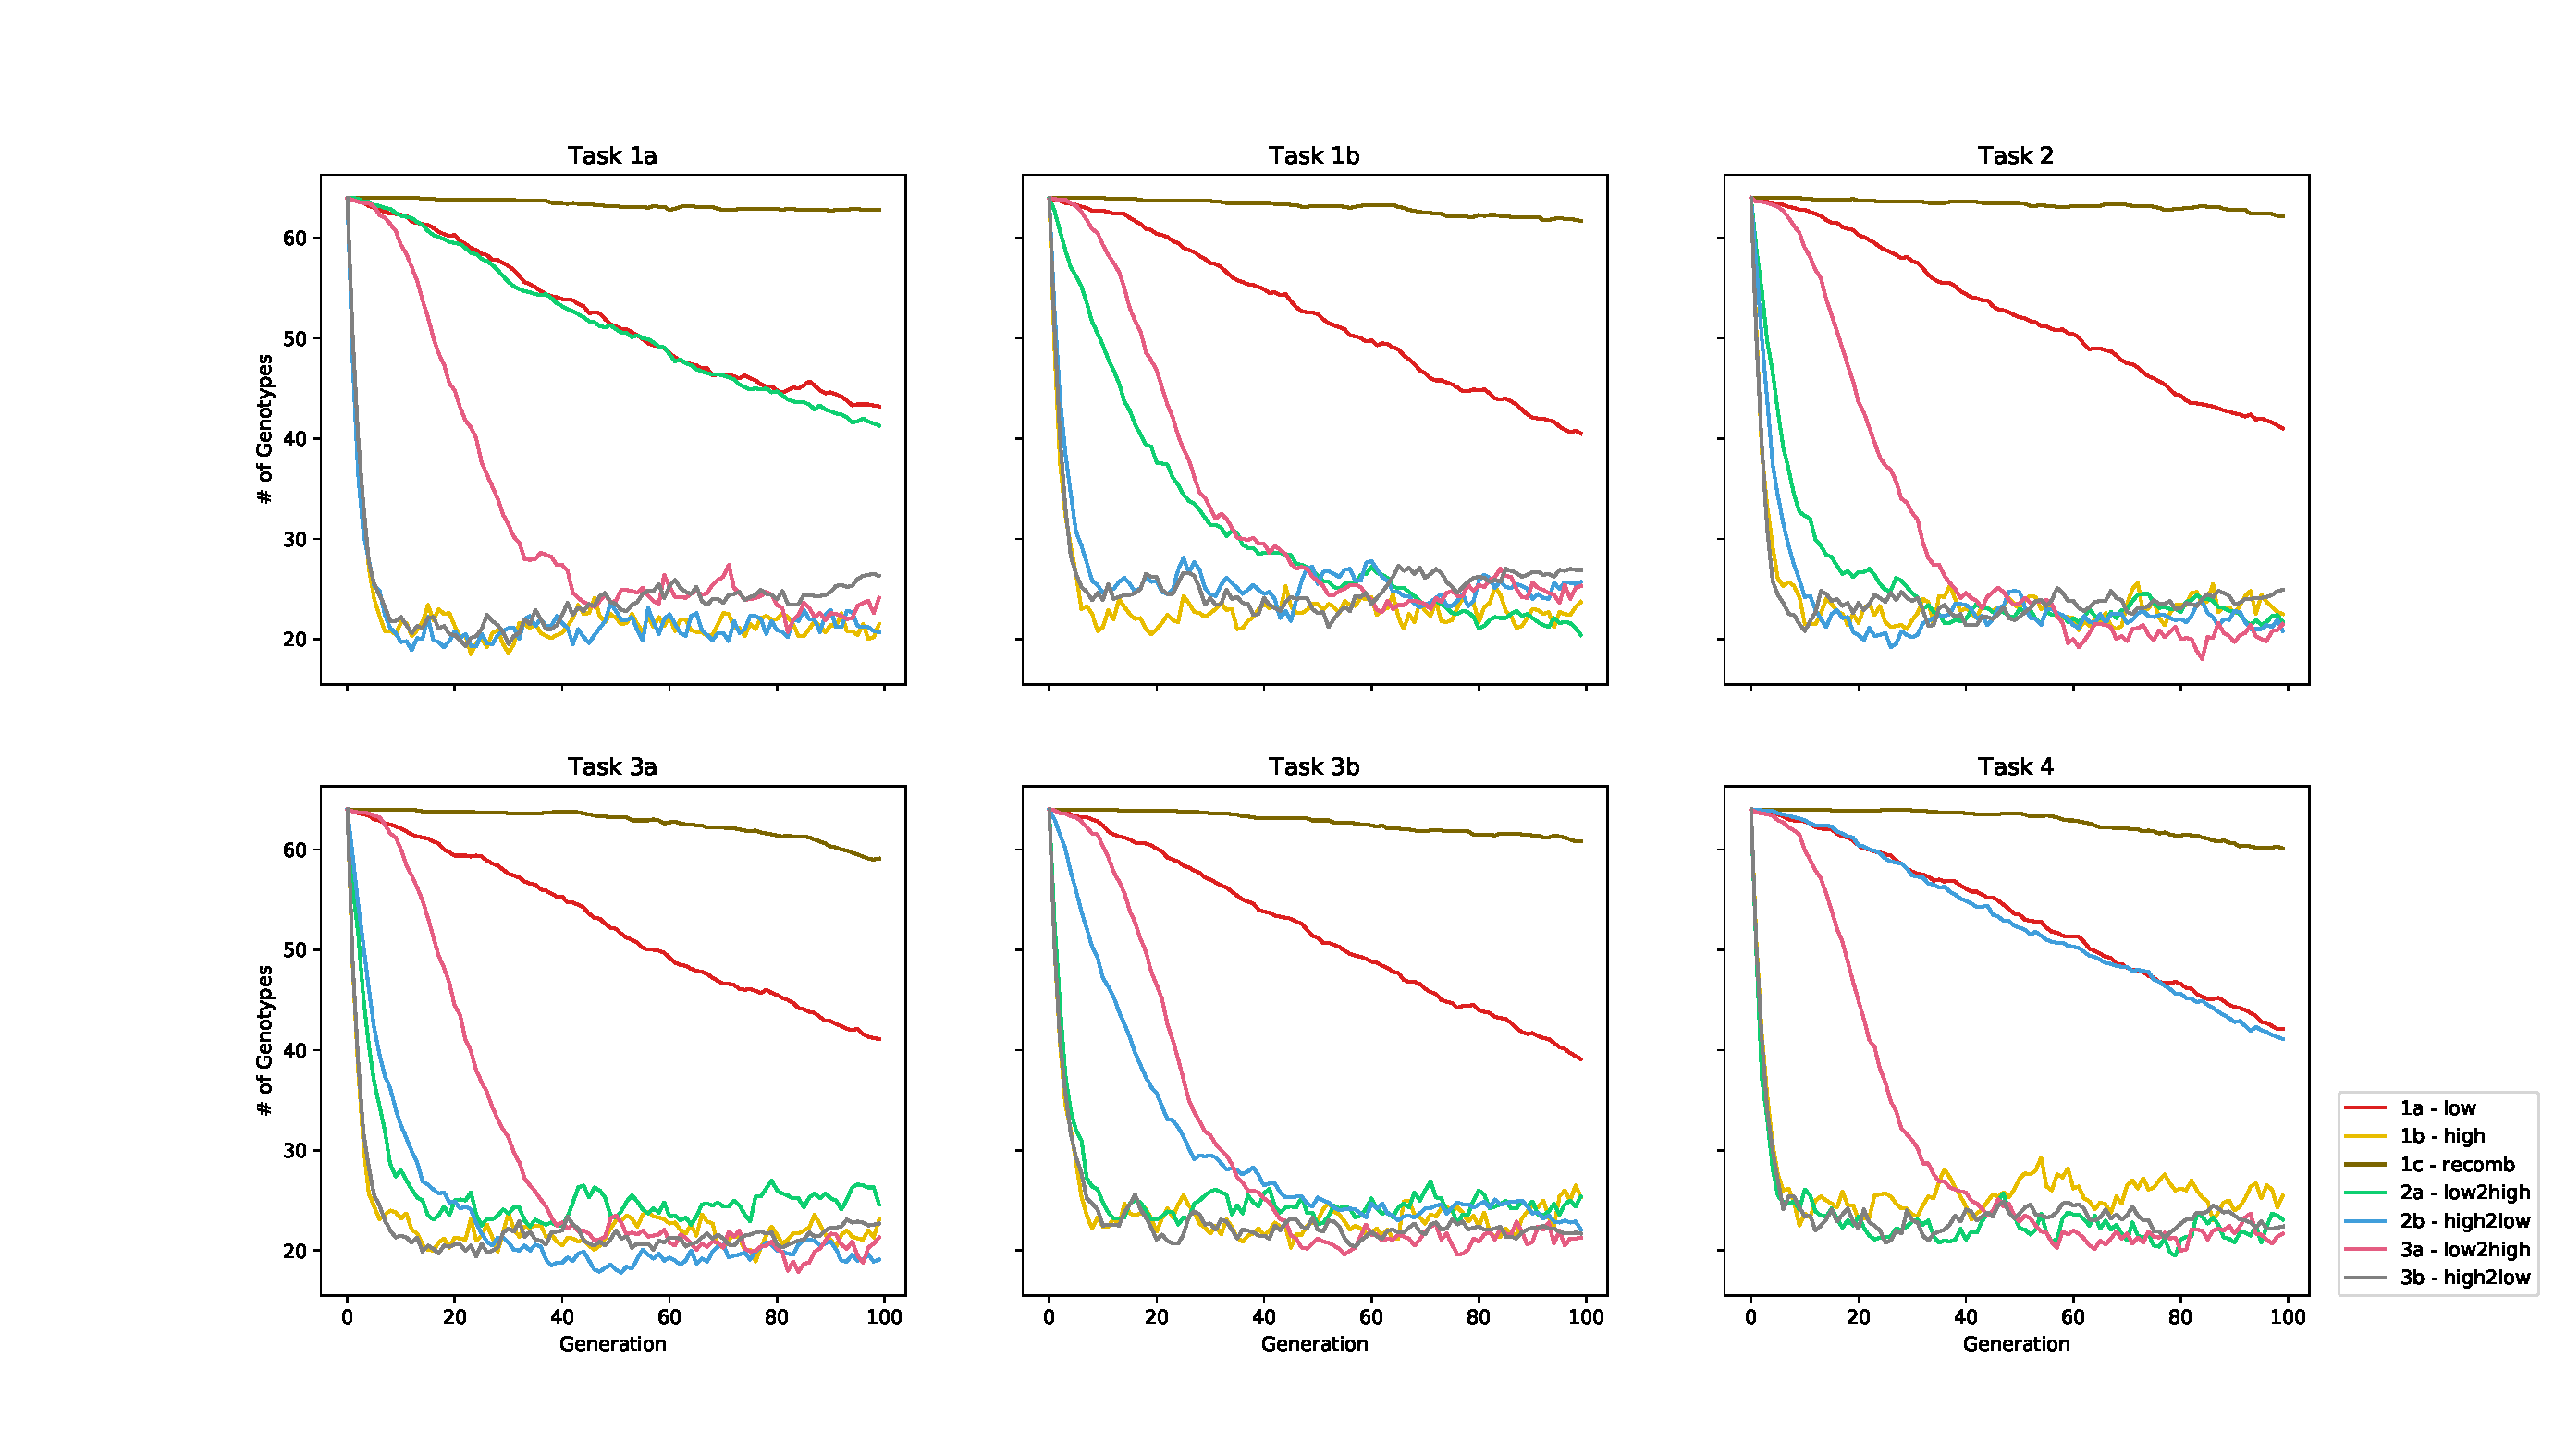
\includegraphics[width=1.2\textwidth,center]{Chapters/4.Experiments/exp2/figures/large/frequency_diversity_unique_path_count.pdf}
    \caption{The number of unique paths within a population. Plotted for every task and every algorithm.}
    \label{fig:search.frequency_diversity_unique}
\end{sidewaysfigure}

Plots \ref{fig:search.hamming_diversity} and \ref{fig:search.frequency_diversity_unique} contain about the same information, and confirms the ordering of selection pressure is what was intended. The only difference worth mentioning is the one of algorithm 1a for the two plots. We would expect the frequency diversity to misrepresent tie diversity of a population as being higher than it actually is due to it counting small mutations as totally different genomes. Here we see frequency giving a smaller diversity than Hamming distance, which suggests Hamming distance is the one misrepresenting reality. 

Also note algorithms 2a and 2b. The convergence rate of these algorithms changes as the tournament size does. Comparing to algorithms 1a and 1b uncovers that tournament size 15, 20 and 25 gives no notable difference in convergence rate from algorithms 1b, while there is a small but visible difference for tournament size 10. Size 5 is the only one distinguishing itself from other tournament sizes or selection pressure schemes. 

Grouping by convergence rate would indicate tournament sizes 10, 15, 20 and 25 are equal to each other and algorithm 3b. 3a is much the same as tournament size 5. 1a is slow but steadily converging and would most likely do so if the generation termination limit was increased, while 1c shows no such tendencies. 

\subsection{Training}

\begin{sidewaysfigure}[p!]
    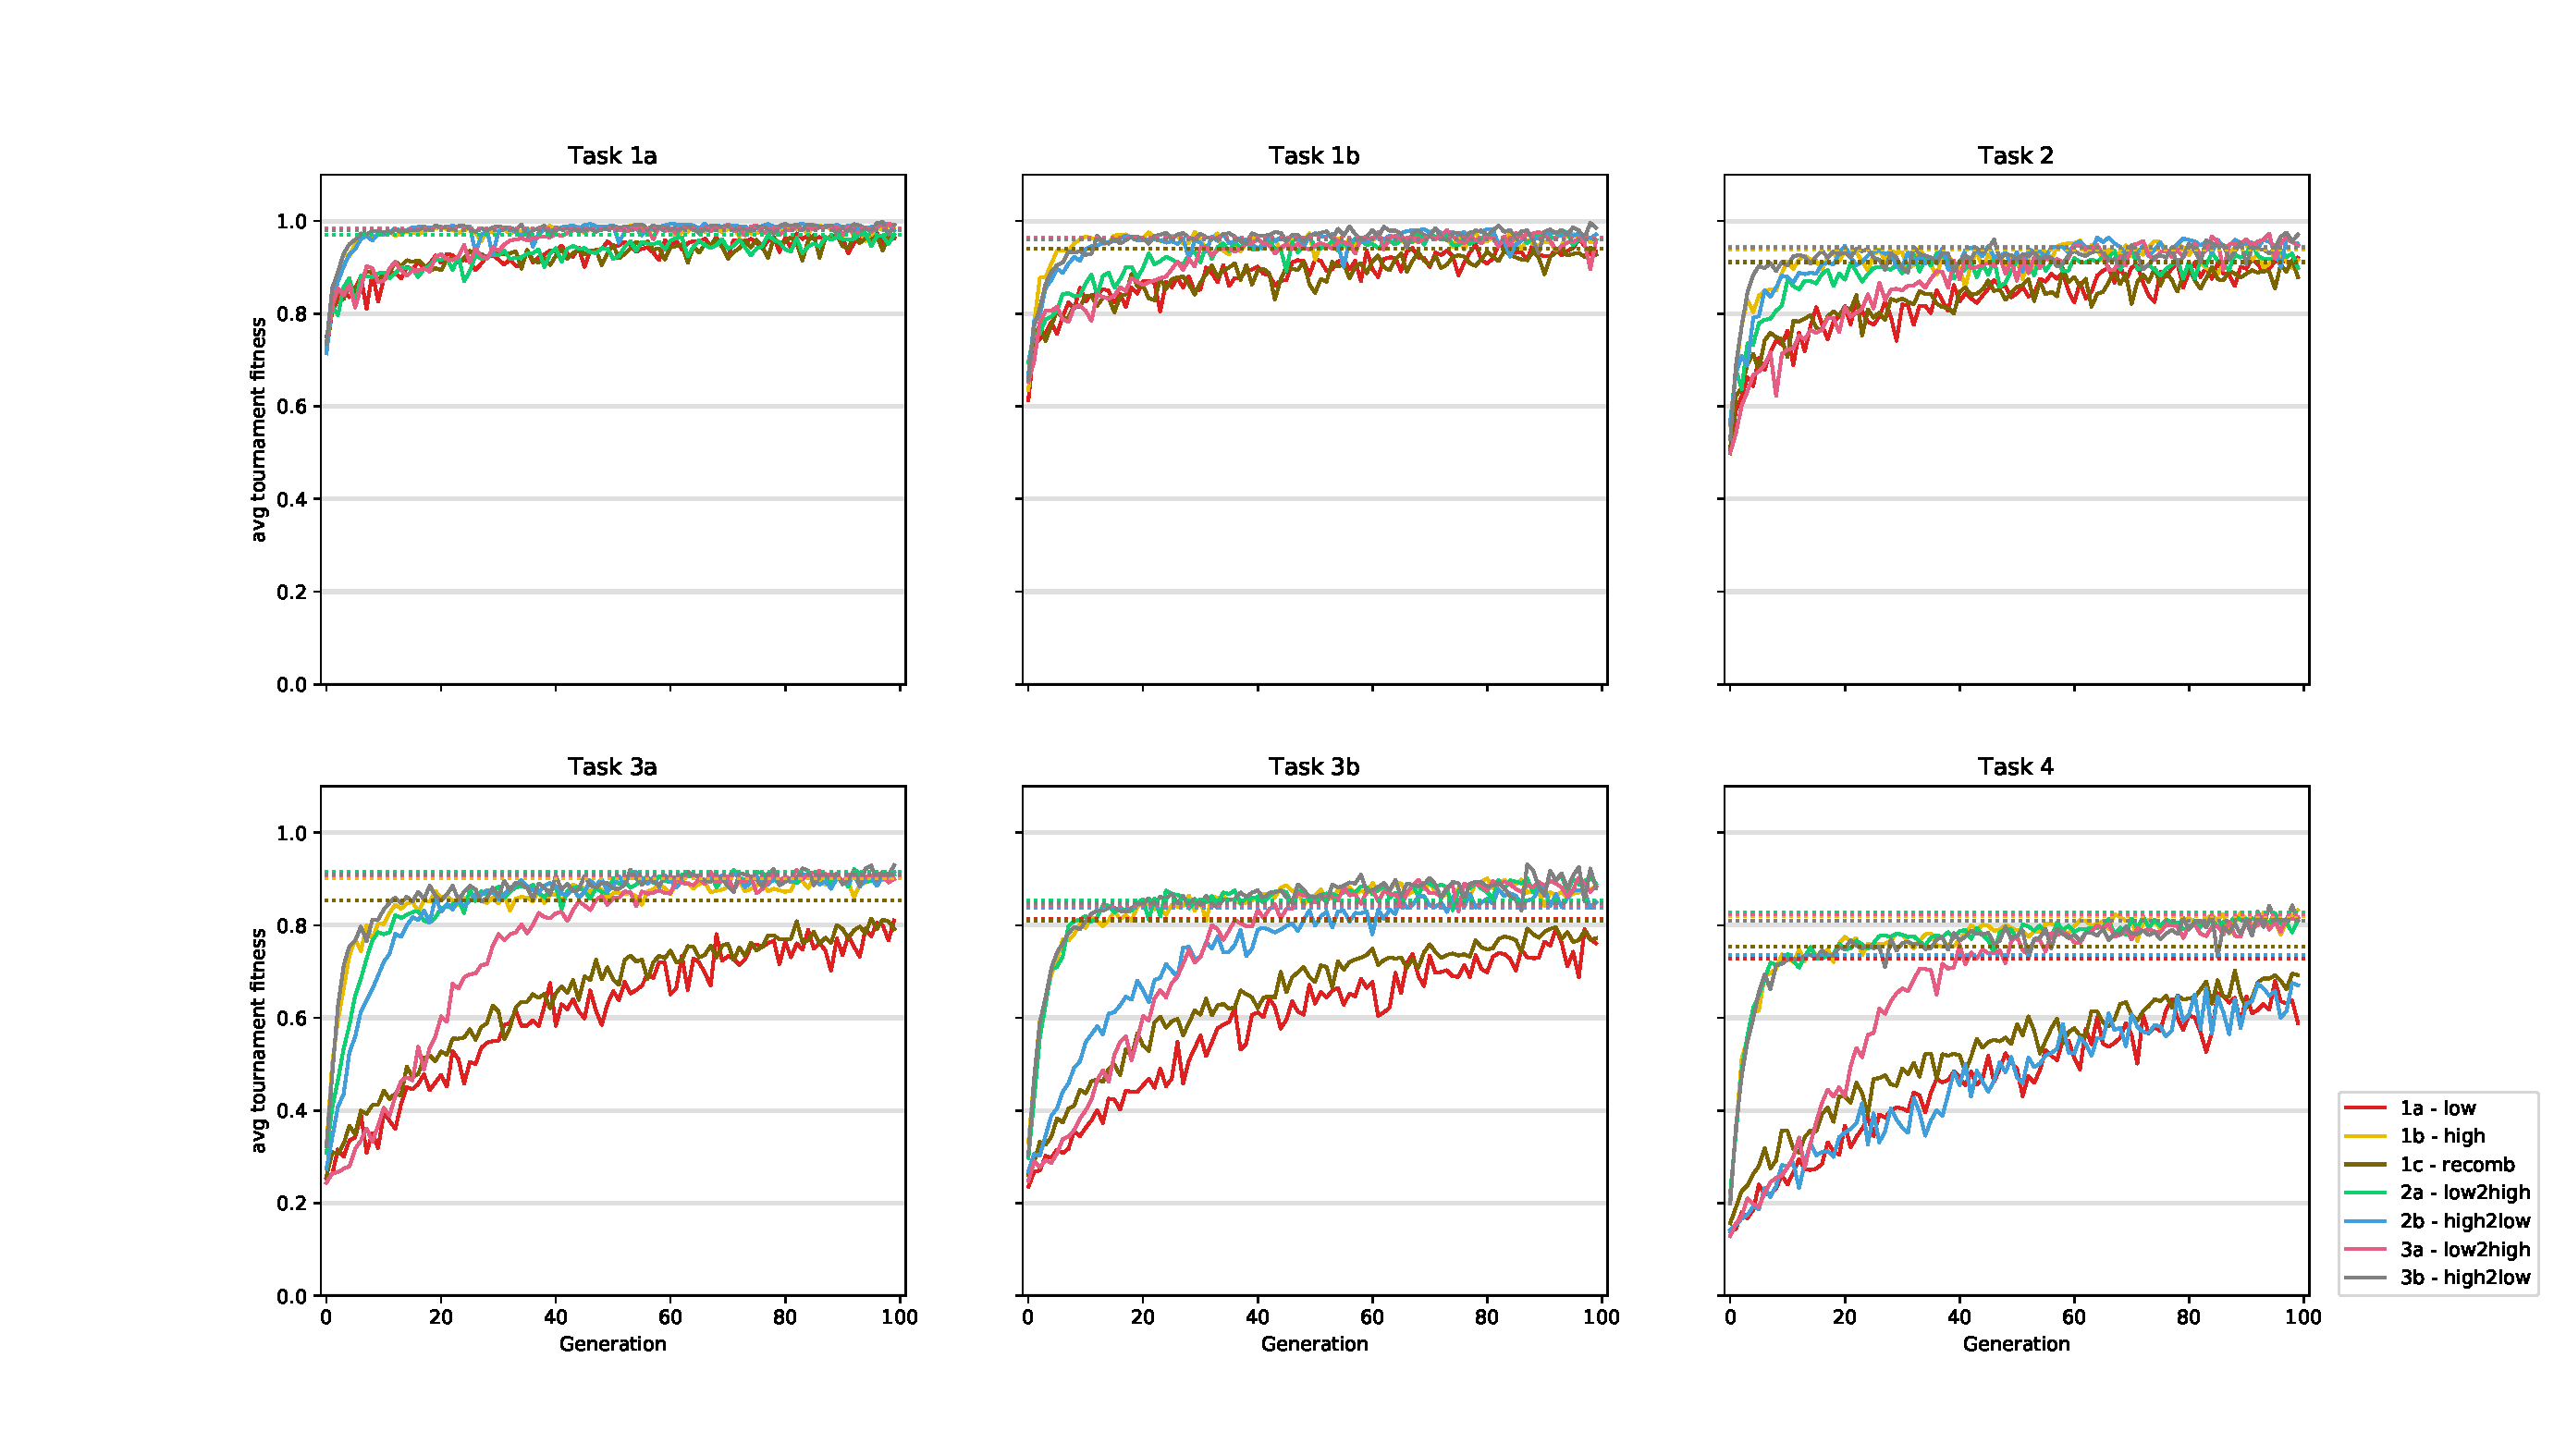
\includegraphics[width=1.2\textwidth,center]{Chapters/4.Experiments/exp2/figures/large/Training_accuracy.pdf}
    \caption{Average training accuracy during search. The dotted lines is the average achieved validation accuracy for that task and that algorithm.}
    \label{fig:search.accuracy}
\end{sidewaysfigure}

As the training of each path is done during and controlled by the search, how the average training accuracy develops gives an indication of how quickly the algorithms are able to influence the overall PathNet to learn a task. As discussed in section \ref{exp2:implementation.search}, the act of training one tournament of genomes effect the previously evaluated fitness values. Because of this, the populations average fitness values would be a highly misleading metric to use and therefore what is plotted in figure \ref{fig:search.accuracy} is the average fitness score achieved within a each generations tournament. Also plotted is the mean validation accuracy reached for each algorithm. This validation score is only calculated after an optimal path have been found for each task, and can therefore not be viewed as a function of generation number. The validation accuracy is visualized separately as a box-plot in figure \ref{fig:search.validation}.

\begin{sidewaysfigure}[p!]
    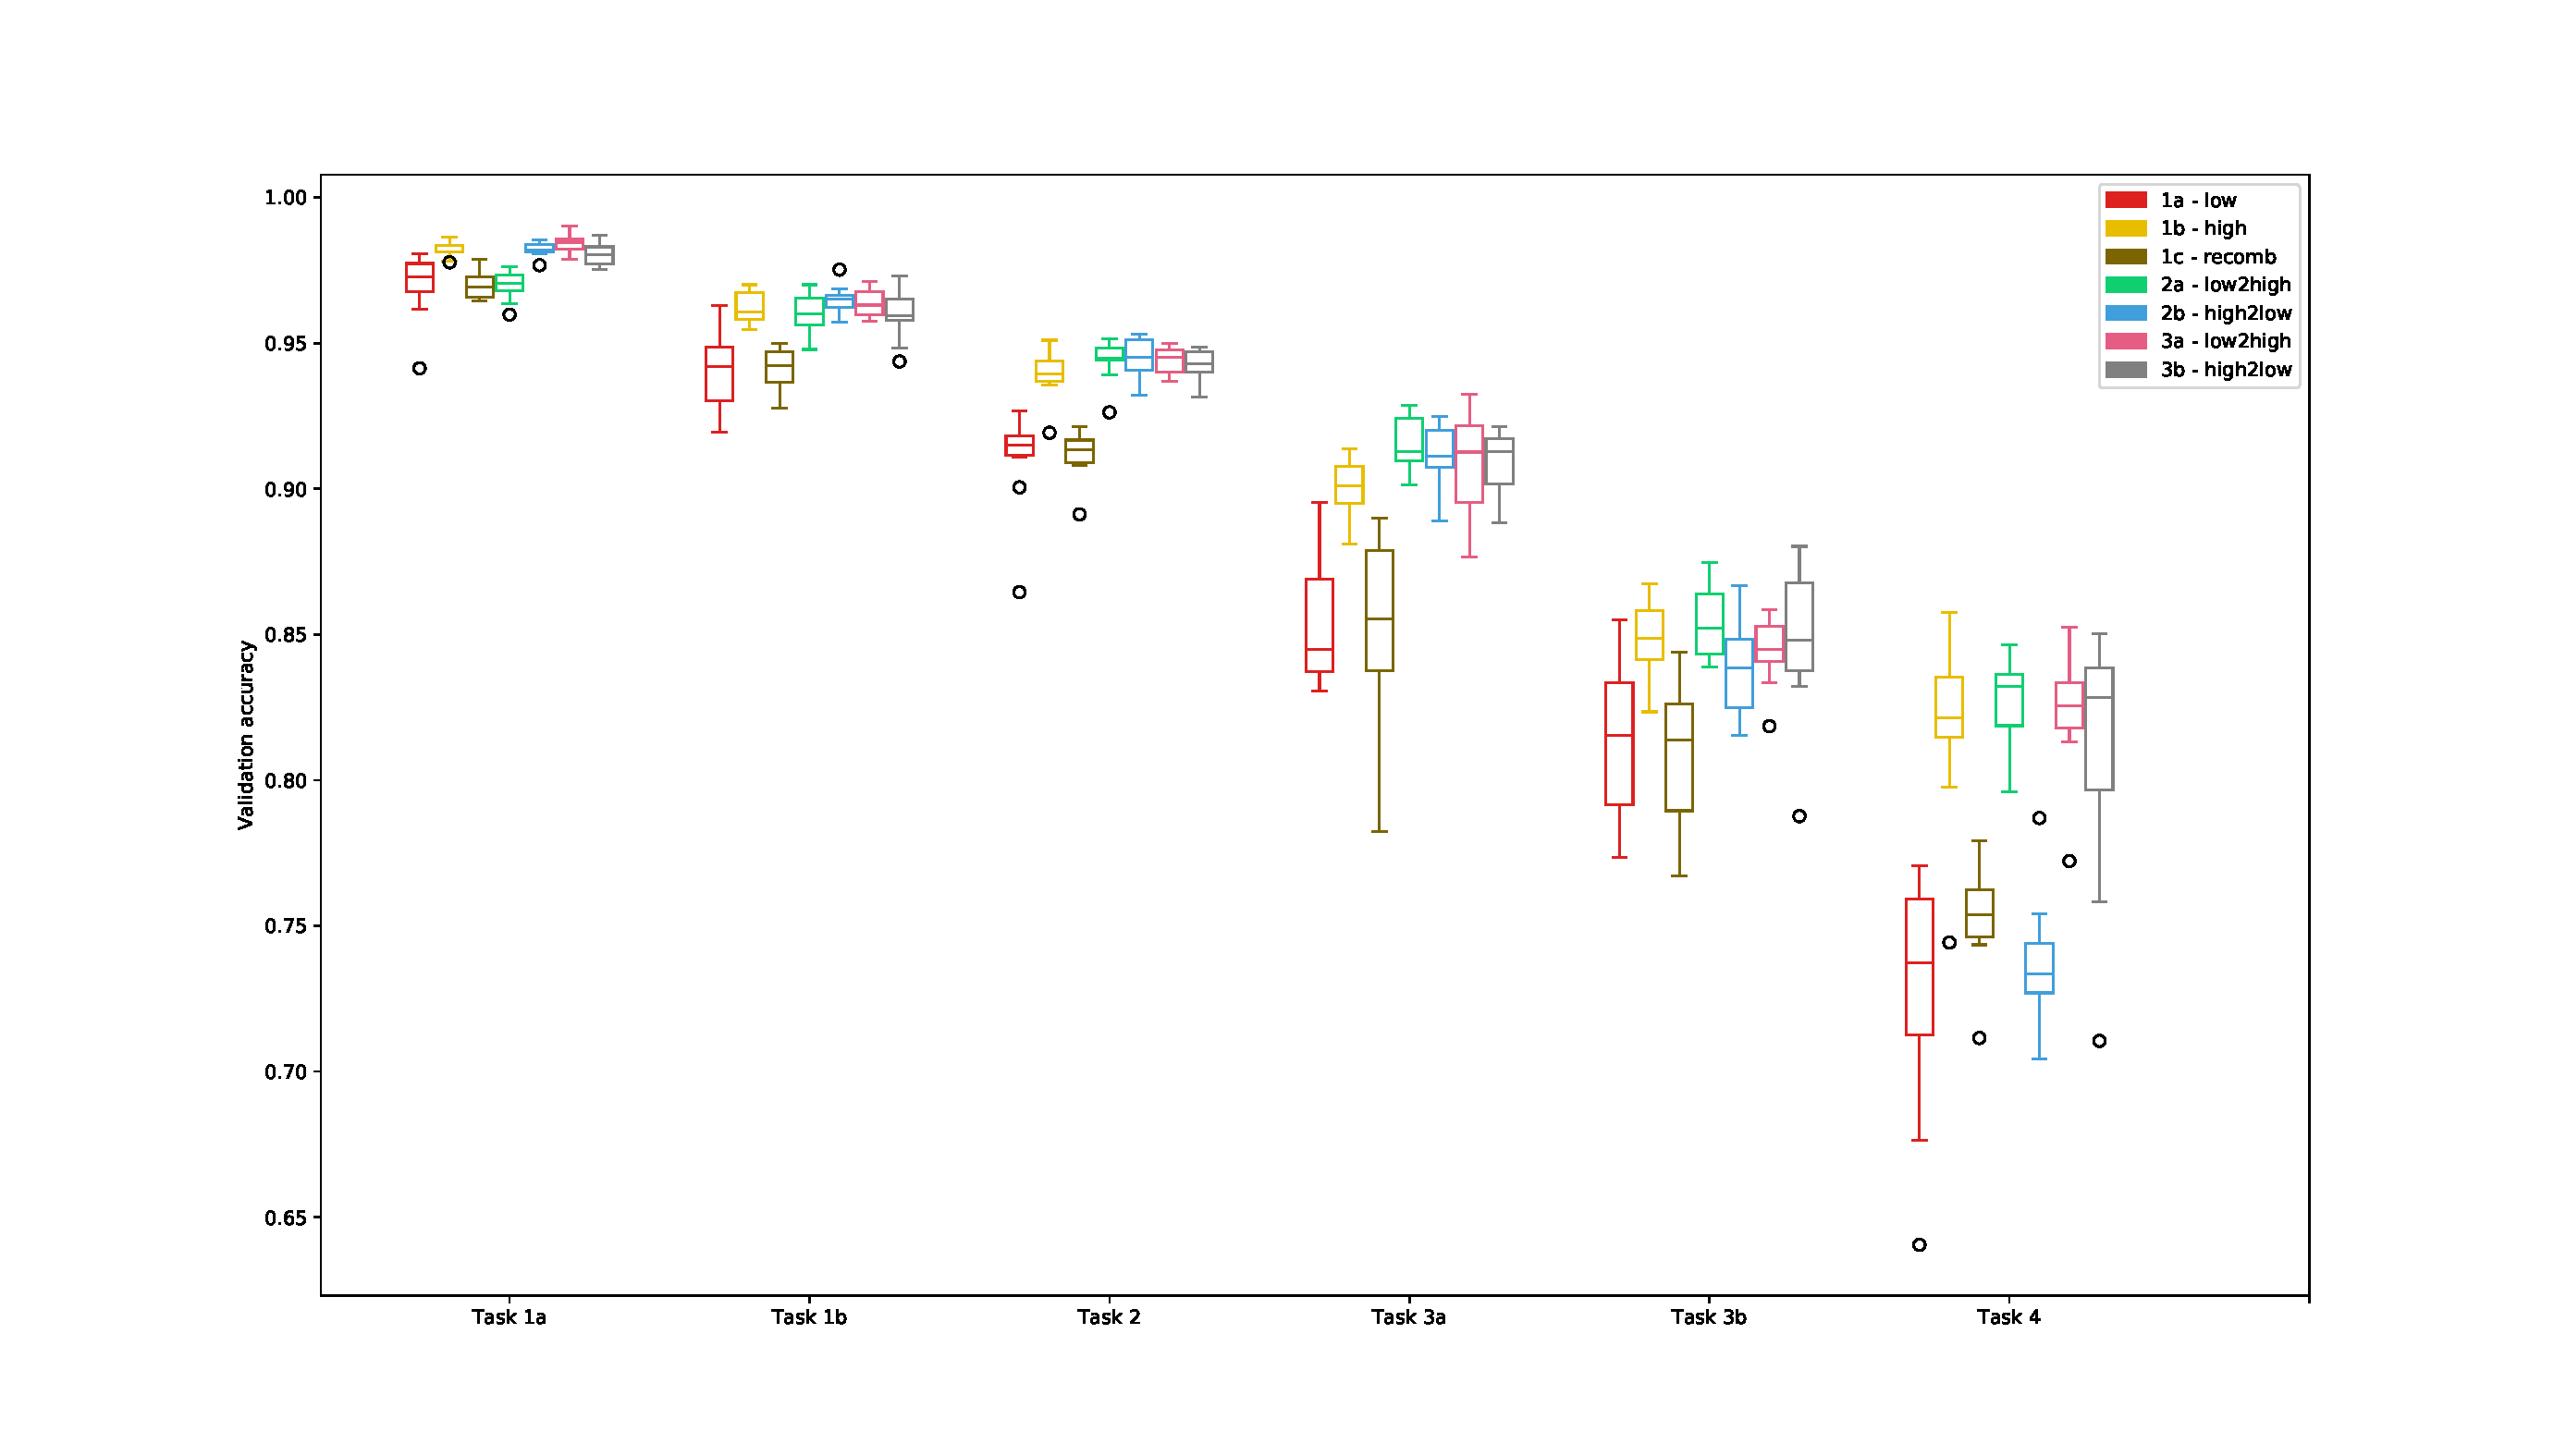
\includegraphics[width=1.2\textwidth, center]{Chapters/4.Experiments/exp2/figures/large/validation_boxplot.pdf}
    \caption{Boxplot of validation accuracy reached for each task and each algorithm.}
    \label{fig:search.validation}
\end{sidewaysfigure}

Again, one MWW-test is run for every pair of algorithm for each task, this time to test the distributions of validation accuracies under the \(\alpha\)-level 0.0003968. Comparing this \(\alpha\) to results in tables in section \ref{appendix:ptable.accuracy}, some patterns emerge: 
\begin{itemize}
    \item Low tournament size: There is no significant difference in accuracy distribution between the algorithms with static low tournament size. The algorithms 2a and 2b are also similar to 1a and 1c for those tasks where they have a low tournament size. Meaning task 1a for algorithm 2a and task 3b and 4 for algorithm 2b. 
    \item High tournament size: Algorithm 1b is only significantly different from other algorithms when they use a tournament size of 2 or 3, the exception being algorithm 1a for task 3b and 4, where the null-hypothesis can not be rejected. 
    \item Changing tournament size: Algorithms 2a and 2b differ significantly only when their tournament size is most different; tasks 1a and 4. 
    \item Dynamic tournament size: Algorithms 3a and 3b does not differ for any task, and are also similar to algorithm 1b for all tasks. They do seem to differ from the low tournament size algorithms for most tasks however, except task 3b. 
\end{itemize}

\begin{sidewaysfigure}[ht]
    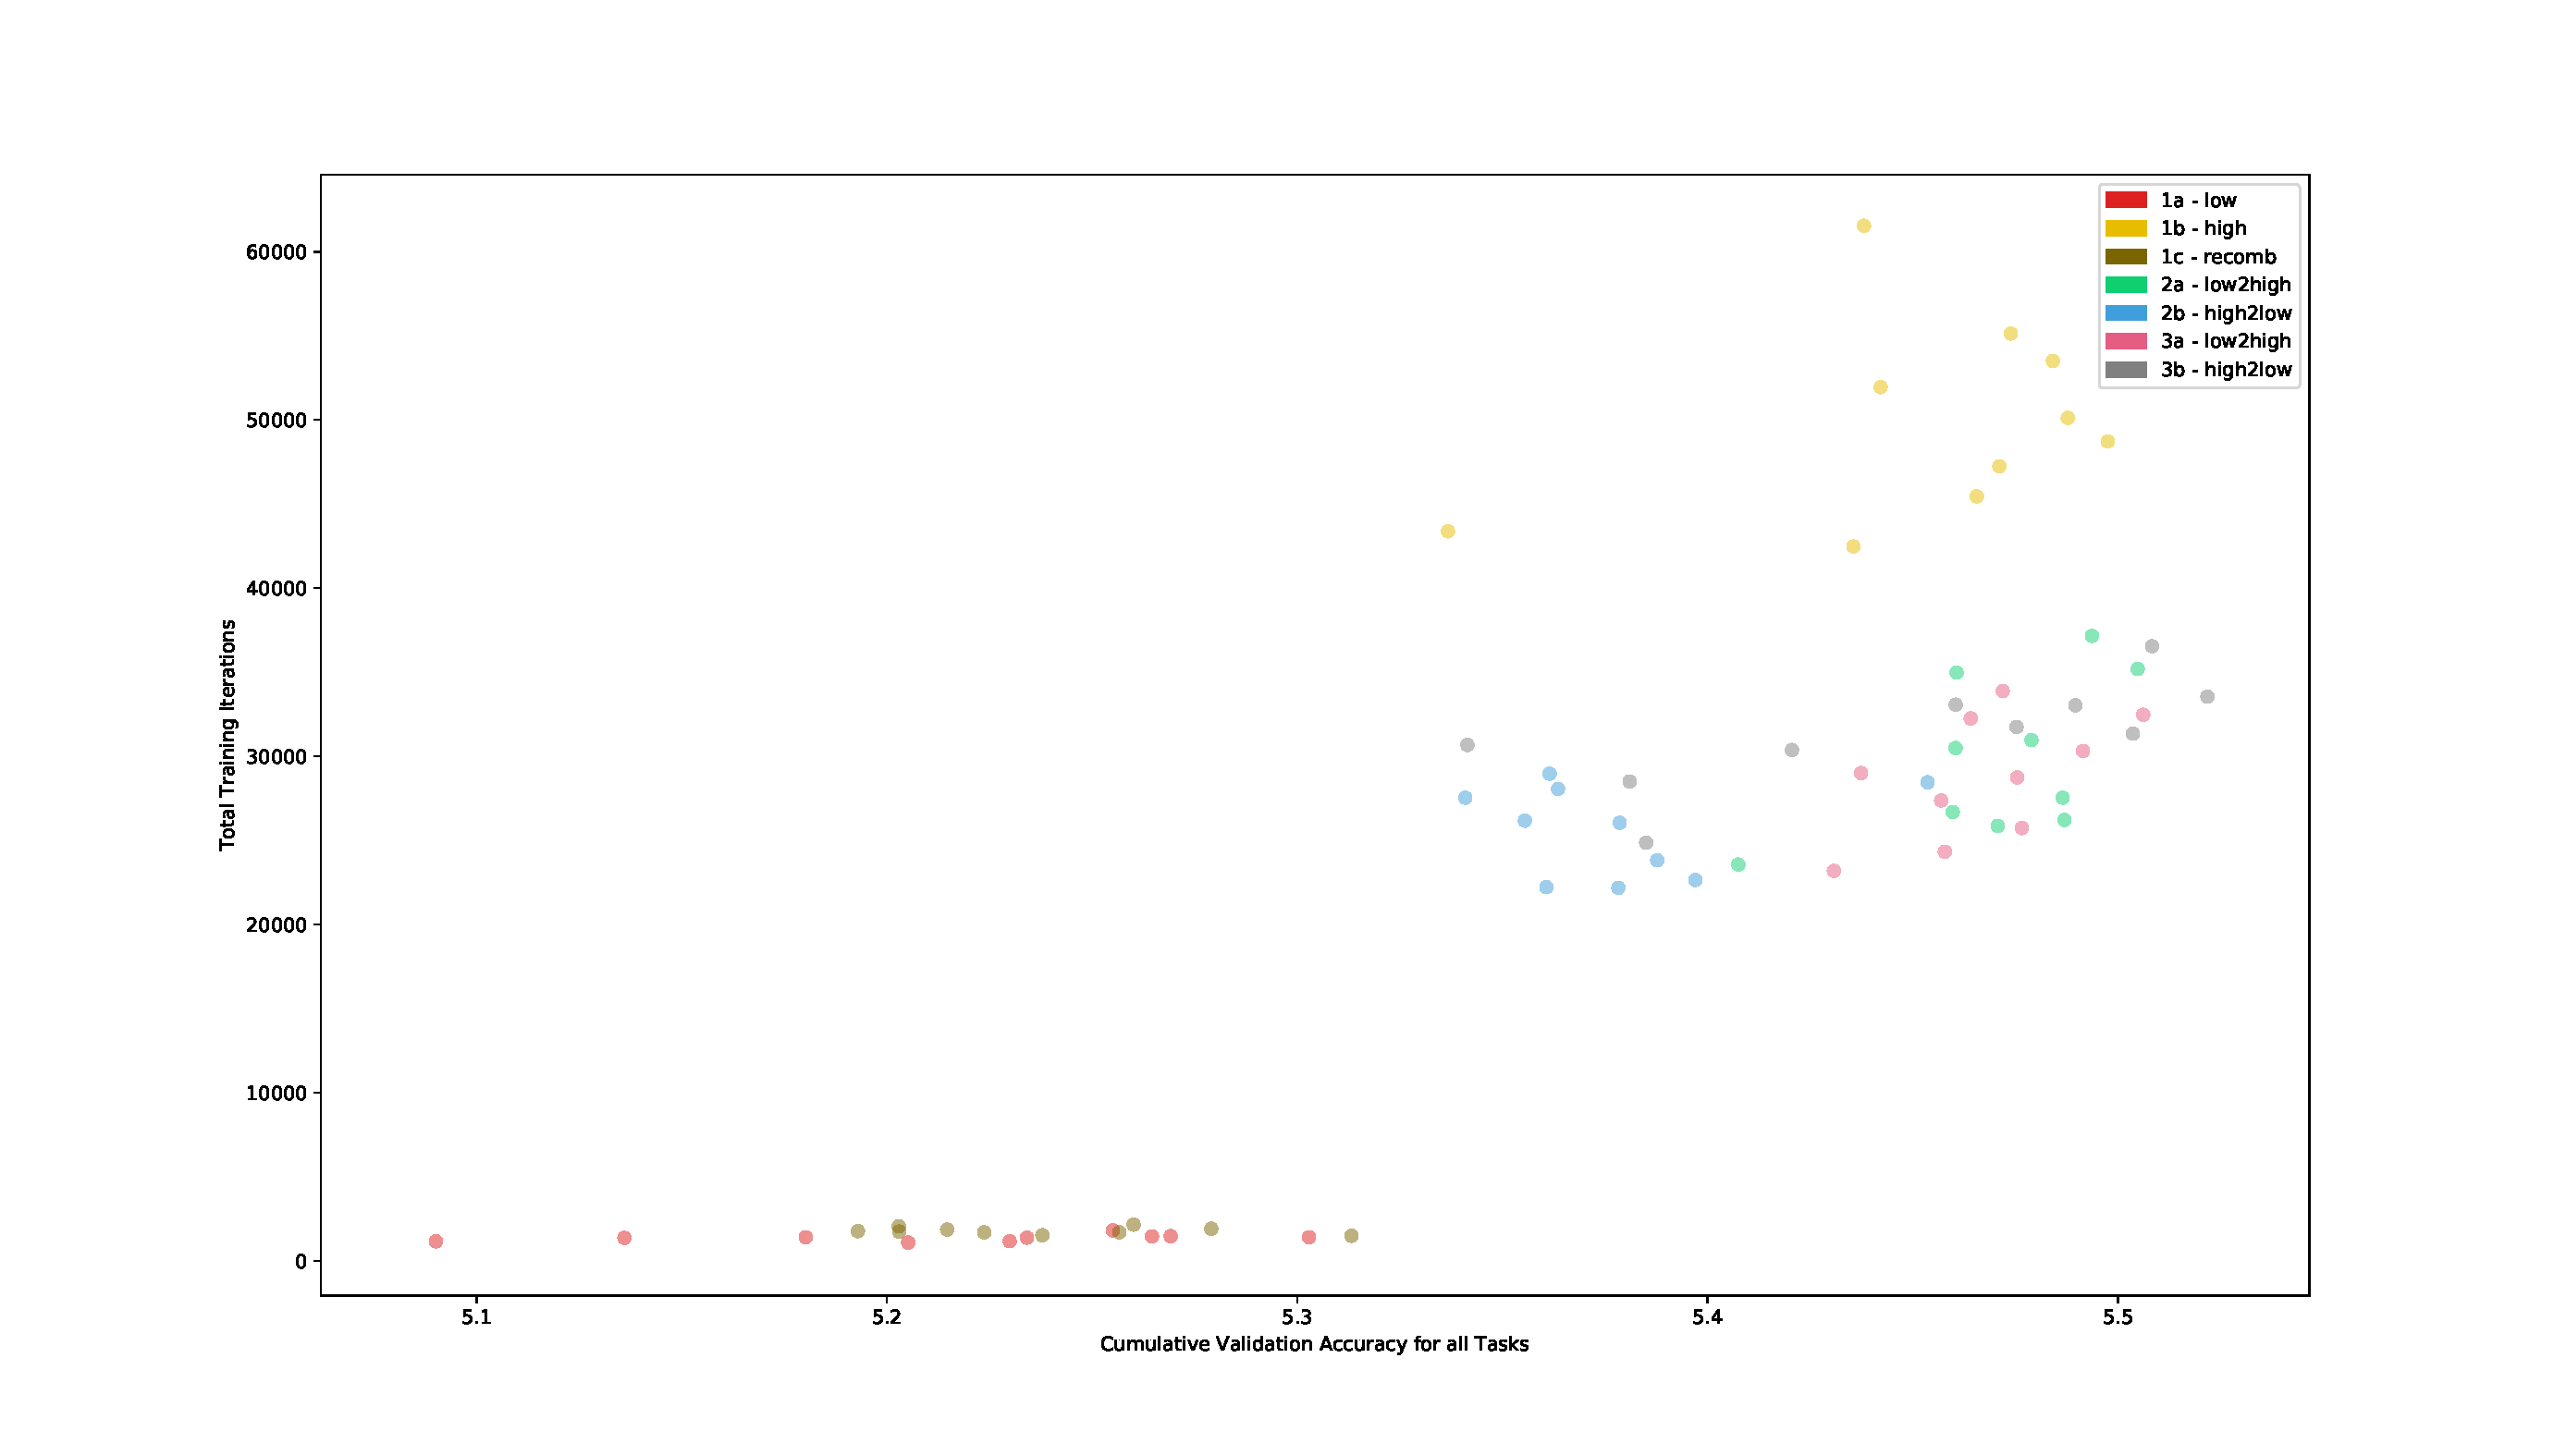
\includegraphics[width=1.2\textwidth,center]{Chapters/4.Experiments/exp2/figures/large/Training_value.pdf}
    \caption{The total amount of training in all optimal paths for each multi-task learning sequence plotted against the cumulative validation accuracy reached for that sequence. The circle size corresponds to the total number of used PathNet modules.}
    \label{fig:search.training_value}
\end{sidewaysfigure}

Training value figure \ref{fig:search.training_value} shows us much of the same as \ref{fig:search.validation}, the difference being the x-axis is the cumulative accuracy reached for all six tasks and the y-axis shows the total amount of training units for all optimal paths found. The circle radius for each trial is correlated to the total use of modules. 

The similarity in performance for algorithms 1a and 1c is present here also, as well as the similarity in validation accuracy for algorithms 1b, 2a, 2b, 3a and 3b. These are separated in training amount, however, which is not surprising as this is highly correlated to the tournament size and this changes between the algorithms. The difference in cumulative accuracy between task 2a and 2b seem to be about 0.1, and can therefore be explained by solely by the difference in validation accuracy between these two algorithms for task 4 as seen in figure \ref{fig:search.validation}. The small tournament size of 2 in algorithms 2b is yields a accuracy around 10 percentage points lower than 2a for this task, giving 2b a lower cumulative score in figure \ref{fig:search.training_value}. Tournament size 2 is still enough to reach a high performance for task 1a, which means this inequality is not equalized when 2a use a low tournament size. 

MWW testing of training amounts does not introduce something not found in plot \ref{fig:search.training_value}. Algorithms 1a, 1b and 1c are significantly different from all other algorithms, including each other. Within the cluster of algorithms 2a, 2b, 3a and 3b, the only pair that differ is 2a and 3b. 

\section{Discussion}
As with the presentation of experimental results, the discussion of these are separated into sections about paths, training and search. 

\subsection{Paths}
While figure \ref{fig:search.reuse} show some differences, the results from these experiments seem to conclude to the different tournament sizes not having any effect on the selection of modules. The results seen here might be different for other tasks however, as a large difference in task difficulty could cause a PathNet starved of capacity to behave differently.

The Monte-Carlo estimated reuse and capacity use was run for \(10^{6}\) trials, making the estimated value accurate to 4 decimal places if holding to a MSE being 1 order of magnitude less than estimates (see formula \ref{eq:montecarloP}). It is noteworthy that ANOVA-tests shows all algorithms mean reuse and mean capacity use can not be separated from each other, but all algorithms perform significantly different from the Mote-Carlo estimates for these metrics. This means we are seeing something similar to experiment in chapter \ref{exp1}, where the tasks were simple enough to learn so modules optimized to quicker to training data than to the interface of pre-trained modules.   

\subsection{Population Diversity}
As hypothesized, low tournament size yielded low convergence rate while high tournament size gave high convergence. Figures \ref{fig:search.hamming_diversity} and \ref{fig:search.frequency_diversity_unique} also makes it possible to rank the algorithms by its selection pressure on a \textit{"exploration vs. exploitation"} scale. Algorithms 2a and 2b change throughout the multi-task scenario, and their selection pressure follow this change. Algorithms 3a and 3b however behave the same for each path-search. From the plots it is obvious that algorithm 3a has a lower convergence rate than 3b as its tournament size starts out small and grows during the search. Meaning 3a has a lower selection pressure than 3b. 

Looking at algorithms 2a and 2b, it seems the tournament size does not scale linearly with convergence. Tournament sizes 10, 15, 20 and 25 have similar convergence rate to that of algorithm 1b. This would indicate that a static tournament size of 10 would provide similar exploration and exploitation to a path search as a tournament size of 25. 

While both algorithm 1a and 1c have low selection pressure and therefor also a low convergence rate, figure \ref{fig:search.frequency_diversity_unique} gives a especially poor image of algorithm 1c as the recombination functionality ensures the offspring is different from both parents and the offspring would not be similar to its parent if not both parents are identical. 

\subsection{Training}
For the three first tasks 1a, 1b and 2 (all based on MNIST) figure \ref{fig:search.accuracy} the tasks are too simple for the algorithms to show any difference as any selection pressure used are capable of reaching a high performance for these tasks. For those based on cSVHN however, a clear split is visible for the algorithms. The split seem to follow the same pattern as the diversity plots \ref{fig:search.hamming_diversity} and \ref{fig:search.frequency_diversity_unique}. The low selection pressure algorithms are steadily increasing in fitness throughout the search and the fitness is still improving when the search terminates, hinting at 100 generations being to little for these algorithms to reach the same performance as those of higher tournament sizes. This is what was hypothesized and is explained by the increase in evaluations (and therefore also training units) for algorithms with higher tournament sizes. The similar fitness progression of 2a and 2b when using tournament size of 10 and higher to that of algorithms 1b, 3a and 3b is interesting however. This points towards performance of tournament size above 10 not being different. Figure \ref{fig:search.validation} supports this suspicions. The ANOVA tests for these results are indeed statistically significant.

When setting this accuracy in context of training in figure \ref{fig:search.training_value} a optimal choice of selection pressure for these tasks are even simpler. A static use of tournament size around 10 would yield a similar performance to that of algorithms 1b, 2a, 2b, 3a and 3b while having a significantly lower training amount than any of these. The training amount used for algorithms 1a and 1c would be even lower, but the performance of a search scheme using tournament size 10 would presumably have a cumulative accuracy around 0.25 points more meaning the hit to computation time could be worth it.  

\section{Conclusion}

The choice of only turning the tournament size dial in these experiments were a conscious one. Parameters such as search termination limit, population size, task-set might lead to other results than those observer here, so ultimately the conclusions drawn are limited by the hyper-parameter space explored. 

Continuation to these experiments should include trials where harder tasks from a more varied domain spectrum are explored. This would encourage using a larger PathNet structure and by increasing the number of allowed module permutations, the search-space increase greatly which again would call for an increase in population size. All these changes brings with it a considerable increase in computational requirements however. 

For these experiments though, the results show a tournament size above 10 is unnecessary. Using this assumption, algorithms 3a and 3b would more than likely perform differently as their increase in selection pressure were intended to be more or less linear, while it here reaches the top level of selection pressure within the first 40\% of each search. As the plot \ref{fig:search.accuracy} show the algorithms with high tournament size max out fitness quite early in the search, the remaining 60\% of the search where algorithm 3a and 3b have functionally the maximum amount of selection pressure should be enough to learn each task, meaning they operate as statically high tournament size algorithms. Changing the range of tournament size these algorithms use would presumably reduce their performance in accuracy to be somewhere between that of 1b and 1a or 1c. Their training amount would decrease also however, so selecting a selection pressure scheme solely based on these metrics might prove to be harder than it is for these results where a static tournament size of 10 seems to be the optimal choice. If the altered size ranges would have a significant effect on module reuse is hard to tell. 

Answering the questions raise in the introduction to this chapter proved to be tougher than originally thought as these experiments only seem to scratch the surface of GA's as optimizer for a Super Neural Network. These results show however, that limiting the tournament size to around 10 can be done for a population size of 64 without taking a hit on performance. Also shown is that tuning the tournament size does shift the search from exploration to exploitation. If this shift affect the search in any significant way should be tested with a harder task-set than used here. 

Also learned during these experiments is how sensitive to method the population diversity is. For debugging and testing search parameters, some combination of pair-wise Hamming distance and a frequency count seem to provide a fair coverage of each methods shortcomings.  

\section{Addendum: Algorithms 3a and 3b}
To verify the change in selection pressure have a effective range from low tournament size for algorithms 1a and 1c and to tournament size 10, algorithms 3a and 3b are run again within this range. MWW tests provided the results found in table \ref{tab:exp2.dynamic_rerun}, where algorithm 3a with the range 2 through 25 is compared to algorithm 3a with range 2 through 10, and the same comparison made for algoritm 3b. 

\begin{table}[h]
    \centering
    \begin{tabular}{llll}
               & Task & \multicolumn{1}{c}{3a} & \multicolumn{1}{c}{3b} \\
    Reuse      & 1b   & 0.956547773748         & 0.956547773748         \\
               & 2    & 0.538144609699         & 0.562088443212         \\
               & 3a   & 0.602834473039         & 1.0                    \\
               & 3b   & 0.757639109903         & 0.696861750189         \\
               & 4    & 0.268673519581         & 0.783737672219         \\
    Validation & 1a   & 0.677126445648         & 0.0279501216272        \\
               & 1b   & 0.939675045144         & 0.448837876623         \\
               & 2    & 0.596563159763         & 0.677470512773         \\
               & 3a   & 0.820463098838         & 0.427181486007         \\
               & 3b   & 0.622390025429         & 0.0815235054997        \\
               & 4    & 0.0539025571694        & 0.650024629906         \\
    Path Size  & 1a   & 0.968962593291         & 0.559304946892         \\
               & 1b   & 0.181629483946         & 0.236641311521         \\
               & 2    & 0.877045299231         & 0.244033263752         \\
               & 3a   & 1.0                    & 0.877045299231         \\
               & 3b   & 0.905680993625         & 0.0624335180351        \\
               & 4    & 0.136097381114         & 0.308603636093        
    \end{tabular}
    \caption{P-values from comparing algorithms 3a and 3b for a tournament size range of \([2,\dots,25]\) with range \([2,\dots,10]\). \(\alpha=1.57\times 10^{-3}\)}
    \label{tab:exp2.dynamic_rerun}
\end{table}

While there is an obvious difference in training units because of the reduced number of evaluations during each search, there is no significant difference in any other tested metrics. Confirming the conclusion that for this case of multi-task problems and PathNet structure, the effective range of tournament sizes spans from the minimum 1\footnote{Tournament size 1 is the same as performing a stochastic search} to 10.